\documentclass{article}
\usepackage[utf8]{inputenc}

\title{curvepy: Bézier Curves, Delaunay Triangulations and Voronoi Diagrams}
%\title{What cagd authors don't want you to know (Number 3.3.5 will suprise you)}
\author{NumerikGang\\Lars Quentin, Maximilian Winkler, Timo Specht}
\date{July 11, 2022}

\usepackage[
backend=biber,
style=alphabetic,
sorting=nyt
]{biblatex}
\addbibresource{paper.bib}

\usepackage{mathtools}
\DeclarePairedDelimiter{\ceil}{\lceil}{\rceil}

\usepackage{graphicx} % for figures
\usepackage{float} % for "H" figure placement
\usepackage{dirtytalk} % quotes
\usepackage{amsmath,amsthm,amssymb,amsfonts}
\usepackage{algorithm}
\usepackage{algpseudocode}
\usepackage[dvipsnames]{xcolor}
\usepackage{cleveref}
\usepackage{setspace} % for \onehalfspacing and \singlespacing macros
\onehalfspacing 
\usepackage{etoolbox}
\AtBeginEnvironment{quote}{\par\singlespacing\small}
\usepackage{caption}
\usepackage{subcaption}
\renewcommand\thesubfigure{\roman{subfigure}}

\newtheorem{definition}{Definition}
\newtheorem{theorem}{Theorem}
\newtheorem{rem}{Remark} [section] 
\newtheorem{lem}{Lemma}
\newtheorem{example}{Example}[section]

\begin{document}
\maketitle
\tableofcontents
\newpage

% the é for free use
\section{Introduction}
\subsection{Motivation}
Computer Aided Geometrical Design, or CAGD, is a branch of numerical mathematics which has a variety of practical applications.\\
Bézier curves are generally utilized to model smooth curves, especially quadratic or cubic ones. They are defined by control polygons and manipulating these polygons results in a change in the original curve. Thus it is quite simple to adjust Bézier curves, which is why they are widely used in computer design, animations, font design, and the car industry. Indeed, Piere Bézier originally invented them to design curves for the bodywork of Renault cars \cite{10.5555/501891}.\\
Constraint Delaunay triangulations are applied in path planning in automated driving and topographic surveying \cite{6232153} and Voronoi diagrams, which are closely related to Delaunay triangulation, are used in fields like biology to model cell \cite{2009arXiv0901.4469B} or bone structures \cite{2012SPIE.8290E..0PL}. More on that later.

\subsection{Scope of this Project}
The main goal of this project was to implement the various algorithms from chapter 3, 4, and 5 of Gerald Farin's book "Curves and Surfaces for CAGD, a pracitcal guide" using Python. That means each mathematical result and formula is taken from this book unless stated differently. \\
The content of chapter 3 focuses on more fundamental topics like linear interpolation or blossoms and served as a great introduction. The most challenging part of not only this chapter but also the entire project was the implementation of an algorithm for the Delaunay triangulation and also the Voronoi diagram.\\
Chapter 4 serves as an introduction to Bézier curves and describes the de Casteljau algorithm. Furthermore it describes properties of Bézier curves and the technique of blossoming. \\
Chapter 5 expands on these topics as it proposes more variations on how one can compute Bézier curves, for instance subdivision and Bernstein polynomials. Moreover different forms of Bézier curves are introduced, namely the monomial and matrix form from which we only focused on the monomial form. At last more properties like the derivative of Bézier curves are established. We decided to not use the matrix form because of its bad conditioning.\\
Since the book didn't contain any definitions on Voronoi diagrams and Delaunay triangulations, this scope extended. We looked at the current literature, evaluated different algorithmic concepts and implemented a \cite{Green1978} based algorithm. 

The project structure can be seen in Figure 1.
\begin{figure}[H]
\centering
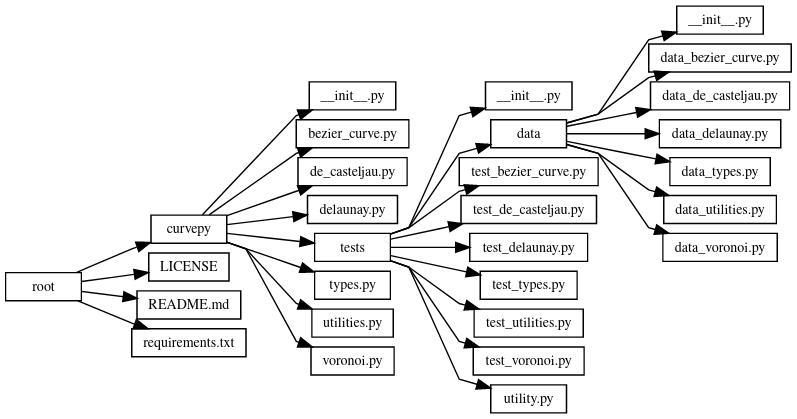
\includegraphics[width=\textwidth]{graphviz.png}
\caption{Project Structure}
\end{figure}
Let us briefly go over the most important architectural design decisions:
\begin{itemize}
    \item[\texttt{requirements.txt}] To keep overhead as minimal as possible we decided to track dependencies via \texttt{requirements.txt} instead of using a more sophisticated build system like \texttt{poetry}.
    \item[\texttt{curvepy}] All Python code is contained within the \texttt{curvepy} top level module, even the tests. This is essential; otherwise any deployment tool (like \texttt{setuptools}) would declare \texttt{tests} as a top level module as well, thus overshadowing any other test module installed within the python environment. Each python file has a has a matching test and data file.
    \item[\texttt{tests}] Our 1000+ test cases, mostly against precomputed and manually verified values contained in \texttt{data}.
    \item[\texttt{\_\_init\_\_.py}] Although most \texttt{\_\_init\_\_.py} files contain no code, they have two specific usages: On the one hand, they contain docstrings which are processed by \texttt{pdoc3} for HTML-documentation. On the other hand, they are required by Python so that the folder is recognized as a module.
    \item[\texttt{LICENSE}] To allow the least restrictive usage of our algorithms, while still keeping ownership of it's interlectual property (unlike public domain licenses like CC-0), we provide all our code as MIT licensed.
    \item[\texttt{README.md}] To provide a simple overview, our library contains a \texttt{README.md}, which can be rendered by Gitlab. 
\end{itemize}
The python files are organized as follows:
\begin{itemize}
    \item[\texttt{bezier\_curve.py}] contains multiple Bézier curve implementations. They all have the same methods; this is done via abstract class inheritance.
    \item[\texttt{de\_casteljau.py}] contains an implementation of the De Casteljau algorithm for computing Bézier curves as well as some utility methods.
    \item[\texttt{delaunay.py}] contains an implementation of a Delaunay triangulation algorithm. It is also used to compute it's dual graph, the Voronoi diagram.
    \item[\texttt{types.py/utilities.py}] contain various helper methods and classes.
    \item[\texttt{voronoi.py}] computes the voronoi diagram through it's underlying Delaunay triangulation.
\end{itemize}
\subsection{Technical Decisions}
Here are some of our technical decisions with their reasoning:
\begin{itemize}
    \item Since we see ourselves as an mostly educational implementation, we formally only support Python 3.8+, although we use \texttt{\_\_future\_\_} imports to keep as much backwards compatibility as possible.\\
    We do not require any complicated version testing tool like \texttt{tox} or building tool like \texttt{poetry}.
    \item Our code style is mostly PEP-8 conform, but with a few exceptions. Here are the according \texttt{flake8}-IDs:
    \begin{itemize}
        \item[\textbf{E731}] \textit{"Do not assign a lambda expression, use a def"}\\
        For single usage methods, we sometimes want to assign a variable name to offer more semantics.
        \item[\textbf{E125}] \textit{"Continuation line with same indent as next logical line"}\\
        This is simply not compatible with PyCharm, which we use as our formatter.
        \item For easier readability, we allow line lengths with up to 120 characters.
    \end{itemize}
    \item For docstrings, we use the \texttt{numpy} docstring format, as we heavily depend on \texttt{numpy} and \texttt{scipy}.
    \item For docstring-based HTML documentation we use \texttt{pdoc3}, since it covers all our use cases while being simpler than sphinx, which requires additional reStructuredText files.
    \item We use \texttt{pytest} for unit tests because it is the most commonly used mature python unit testing framework.
    \item For formatting, we use Jetbrains default formatter, which is shipped with PyCharm.\\
    Additionally, we use \texttt{isort} for import ordering.
    \item Once we publish our library on PyPI, we will use version numbers according to PEP 440.\\
    Note that this is \textit{not} compatible with Semantic Versioning (SemVer).\\
    Further note that this prohibits git-hashes as version numbers since they have no formal ordering.
\end{itemize}
We also use the continuous integration (CI) provided by Gitlab. Specifically, we use the default Gitlab runner provided by the GWDG. Our pipeline is split into 3 stages:
\begin{itemize}
    \item[\texttt{static-analysis}] We use \texttt{flake8} as our linter. \texttt{flake8} is a combination of \texttt{pep8}, which checks conformity against the PEP 8 design standard, as well as \texttt{pyflakes}, which provides a substantial amount of plugin functionality.\\
    We use the following extensions:
    \begin{itemize}
        \item \texttt{flake8-bugbear} "A plugin for Flake8 finding likely bugs and design problems in your program."
        \item \texttt{pep8-naming} "Check your code against PEP 8 naming conventions."
        \item \texttt{flake8-builtins} "Check for python builtins being used as variables or parameters."
        \item \texttt{flake8-comprehensions} "A flake8 plugin that helps you write better list/set/dict comprehensions."
    \end{itemize}
    \item[\texttt{test}] On every commit to \texttt{master} as well as merge requests we run our full \texttt{pytest} based test suite.
    \item[\texttt{deploy}] After every commit to \texttt{master}, we automatically update and redeploy our HTML based documentation \cite{CPY}.
\end{itemize}
\subsection{Acknowledgements}
Firstly, we want to thank Dr. Jochen Schulz and Prof. Dr. Gerlind Plonka-Hoch for their monumental patience, waiting around 2 years for this project to complete.\\
Secondly, we want to thank Gerald E. Farin for his detailed overview of computer aided graphic design \cite{10.5555/501891} and Franz Aurenhammer and Steven Fortune for their great meta analysis of Voronoi and Delaunay research \cite{Aurenhammer1991} \cite{FORTUNE1995}.\\
Lastly, we want to thank the now defunct "Coffeebar ins Grüne" for all the great Currywursts which were soaked in a comically large amount of oil that would make any government jealous.
\newpage
\section{Bézier Curves}
First we will go over some preliminaries that are useful to know before we get to actual Bézier curves. Then we introduce the general concept of Bézier curves and give an overview how we implemented the different methods to calculate Bézier curves followed by detailed sections about these methods and their implementation.
\subsection{Linear Interpolation}
\begin{definition}(Straight Line)
Let $a, b \in \mathbb{R}^2$ be 2 points. A \textbf{straight line} is defined as the set of all possible combinations
\[x = x(t) = (1-t) \cdot a + t \cdot b\]
where $t \in [0,1]$.
\end{definition}
But we can also express $t$ as $t=(1-t) \cdot 0 + t \cdot 1$. Hence $t$ is also just a point lying on a straight line between $0$ and $1$ and therefore the points $a,x,b$ are an \textbf{affine map} on $0,t,1$.
\begin{definition}(Linear Interpoaltion)
\textbf{Linear interpolation} is an affine map of the real line onto a straight line.
\end{definition}
Since we see linear interpolation as an affine map we get the following property.
\begin{definition}
Linear interpolation is \textbf{affine invariant}. Thus the following holds
\[\phi(x) = \phi((1-t) \cdot a + t \cdot b) = (1-t) \cdot \phi(a) + t \cdot \phi(b)\]
where $\phi$ is an affine map, $t \in [0,1]$ and $a,b$ are two points in $\mathbb{R}^2$.
\end{definition}


\subsection{Piecewise Linear Interpolation}
% Mein Vorschlag
\begin{definition}(Polygon)
A \textbf{Polygon} is defined as a finite sequence of points $b_0,\dots,b_n \in \mathbb{R}^m$ where each two consecutive points $b_i$ and $b_{i+1}$ are connected by a straight line.\\
\end{definition}
With this we can define the piecewise linear interpolant of a curve $c$.
\begin{definition}(piecewise linear interpolant)
Let $c$ be a curve. The polygon interpolating the $b_i$ is the \textbf{piecewise linear interpolant} $PL$ of $c$ if and only if all points lie on $c$.
\end{definition}
\begin{rem}
One can easily show that the piecewise linear interpolant is \textbf{affinely invariant}, which means that for any curve $c$ and affine map $\phi$
\[
PL(\phi(c)) = \phi(PL(c))
\]
\end{rem}


\subsection{Menelaos' Theorem}
\begin{theorem}\label{Men}
Let $b$ be an open polygonal chain of $b_0, b_1, b_2 \in \mathbb{R}^2$.  We can define any points on the straight lines as convex combinations of those points.
\begin{align*}
    b[0,t] &= (1-t) \cdot b_0 + t \cdot b_1\\
    b[s,0] &= (1-s) \cdot b_0 + s \cdot b_1\\
    b[t,1] &= (1-t) \cdot b_1 + t \cdot b_2\\
    b[s,1] &= (1-s) \cdot b_1 + s \cdot b_2\\
\end{align*}
Where $s,t \in [0,1]$ and $b[*, *]$ is a two-dimensional blossom (we will talk more about blossoms in the next section). With this we define $b[s,t], ~ b[t,s]$ as:
\begin{align*}
    b[s,t] &= (1-t) \cdot b[s,0] + t \cdot b[s,1]\\
    b[t,s] &= (1-s) \cdot b[0,t] + s \cdot b[t,1]
\end{align*}
Menelaos' theorem now simply states
\[
    b[s,t] = b[t,s]
\]
\end{theorem}
\begin{proof}
\begin{align*}
    b[s,t] &= (1-t) \cdot b[s,0] + t \cdot b[s,1]\\
    &= (1-t) \cdot ( (1-s) \cdot b_0 + s \cdot b_1 ) + t \cdot ( (1-s) \cdot b_1 + s \cdot b_2 ) \\
    &= (1-t) \cdot (1-s) \cdot b_0 + (1-t) \cdot s \cdot b_1 + t\cdot (1-s) \cdot b_1 + t \cdot s \cdot b_2\\
    &= (1-t) \cdot (1-s) \cdot b_0 + t\cdot (1-s) \cdot b_1 +  (1-t) \cdot s \cdot b_1 +t \cdot s \cdot b_2\\
    &= (1-s) \cdot ( (1-t) \cdot b_0 + t \cdot b_1 ) + s \cdot ( (1-t) \cdot b_1 + t \cdot b_2 )\\
    &= (1-s) \cdot b[0,t] + s \cdot b[t,1]\\
    &= b[t,s]
\end{align*}
\end{proof}
This means that the resulting point is continuous linear interpolation is invariant to the order of weights used.
\begin{figure}[H]
    \centering
    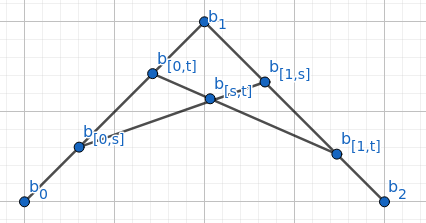
\includegraphics[width=15em]{Menelaos3.png}
    \caption{Points defined on the straight line of our previously defined points}
    \label{fig:Men}
\end{figure}
\subsection{Blossoming}
\begin{definition}(Blossoms)
\textbf{Blossoms} are a multivariate function. Denoted $b[t_1, \dots, t_n]$, where $t_i \in \mathbb{R}$ for $i \in \{1, \dots, n\}$. 
\end{definition}
So in each interpolation step a different $t$ can be used.
Blossoms have some very interesting properties that are useful for types of Bézier curves:
\begin{lem}\label{sym}(\textbf{Symmetry})
In the case of Blossoms the order of the arguments does not change anything; in fact this is an application of \cref{Men}:
\[b[t_1, \dots, t_n] = b[\pi(t_1, \dots, t_n)]\]
where $\pi(t_1, \dots, t_n)$ denotes some permutation matrix and $t_i \in \mathbb{R}$ for $i \in \{1, \dots, n\}$.
\end{lem}
Before we can look at the next property let us fist define \textbf{Multi Affinity} and \textbf{barycentric combinations}.
First we will define multi affinity.
\begin{definition}(Multi Affinity)
A function is \textbf{multi affine} if it is affine in regards to every parameter.
\end{definition}
Now let us introduce barycentric combinations.
\begin{definition}
Let $P_1, \dots, P_n$ be points in $\mathbb{R}^m$ and $\alpha_1, \dots, \alpha_n$ be weights in $\mathbb{R}$.
A \textbf{barycentric combination} of the points $P_1, \dots P_n$ is a weighted sum\[\sum_{i=1}^n \alpha_i \cdot P_i\] with the affinity constraint
\[\sum_{i=1}^n \alpha_i = 1\]
\end{definition}
 Before we look at the general case, let us examine a simple example:
\[b[\alpha \cdot r + \beta \cdot s, t_2] = \alpha \cdot b[r, t_2] + \beta \cdot b[s, t_2]\]
So if the first argument is a barycentric combination, we can compute the blossom values separately and then build the barycentric combination. Of course we are not restricted to the case for the first argument, since we have symmetry. In general we have:
\begin{lem}(\textbf{Multi Affinity})
\[b[\alpha \cdot r + \beta \cdot s, *] = \alpha \cdot b[r, *] + \beta \cdot b[s, *]\]
where $\alpha + \beta = 1$, $r,s \in \mathbb{R}$ and $*$ denotes the same arguments. However the order of the parameters does not play a role, as shown in \cref{sym}.
\end{lem}
\begin{rem}(\textbf{Diagonality})
Let $t = t_1 = \dots = t_n$ and $t_i \in \mathbb{R}$ for $i \in \{1, \dots, n\}$. In this case we obtain a polynomial curve or Bézier curve. We use the notation:
\[b[t, \dots, t] = b[t^n]\]
if the argument $t$ is repeated $n$ times.
\end{rem}
\newpage
\subsubsection{Leibniz Formula}
If we use the properties we just defined we can consider a special case where we have $(\alpha \cdot r + \beta \cdot s)$ $n$ times as argument. We get:
\begin{lem}\label{leib}(\textbf{Leibniz Formula)}
\[b[(\alpha \cdot r + \beta \cdot s)^n] = \sum_{i=0}^n \binom{n}{i} \alpha^{i} \cdot \beta^{n-i} \cdot b[r^{i}, s^{n-i}]\]
\end{lem}
\subsection{Definition of Bézier Curves}
Before we will have a look at different types of Bézier Curves and how they can be calculated. Let us first define what a Bézier Curve is.
\begin{definition}
A \textbf{Bézier curve} is a parametric curve described by control points $b_0, \dots, b_n \in \mathbb{R}^2$. These points form the so called Bézier polygon or control polygon the $b_i$ are called \textbf{Bézier points} or \textbf{control points}, and we use these terms interchangeably. The degree of the curve described by the polygons is $n-1$. \\
\end{definition}
The actual Bézier curve can be formed using a variety of different formulas that all use some weight $t$, which is normally on the unit interval, on the Bézier points. So we write $b_0^n(t)$ for an actual point on the curve and $b_i^0(t) := b_i$ for the Bézier points, similar to the notion we already used in the blossom section.

\begin{figure}[H]
    \centering
    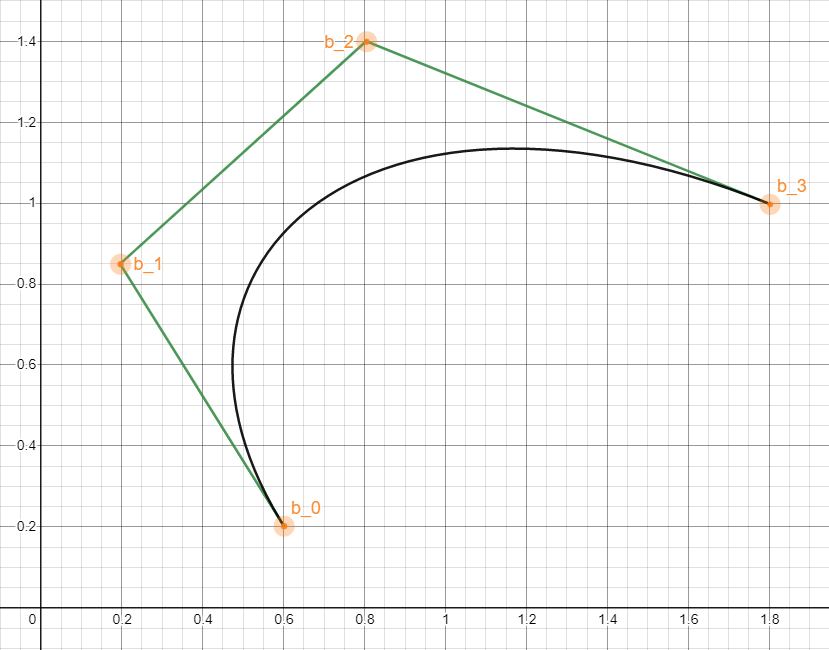
\includegraphics[width=0.7\textwidth]{Beispiel_Bezierkurve.png}
    \caption{Example Bézier curve with control polygon}
    \label{fig:my_label}
\end{figure}

\subsection{General Implementation of Types of Bézier Curves}
To implement the different types of Bézier curves we use a clever class hierarchy. \\

% picture here
We use an abstract class as our base. This one implements most of the methods all of its children use. Like the derivative, addition, multiplication and so on. \\

The most fundamental function is the curve function, which is a cached property. Calling this method generates the preferred amount of evaluated points for the given Bézier points. The curve function supports either parallel or serial execution.\\

The curve is based on the abstract \texttt{init\_func}, which is the only method that needs to be provided by any subclass. This makes inheritance very elegant.

\begin{figure}[H]
    \centering
    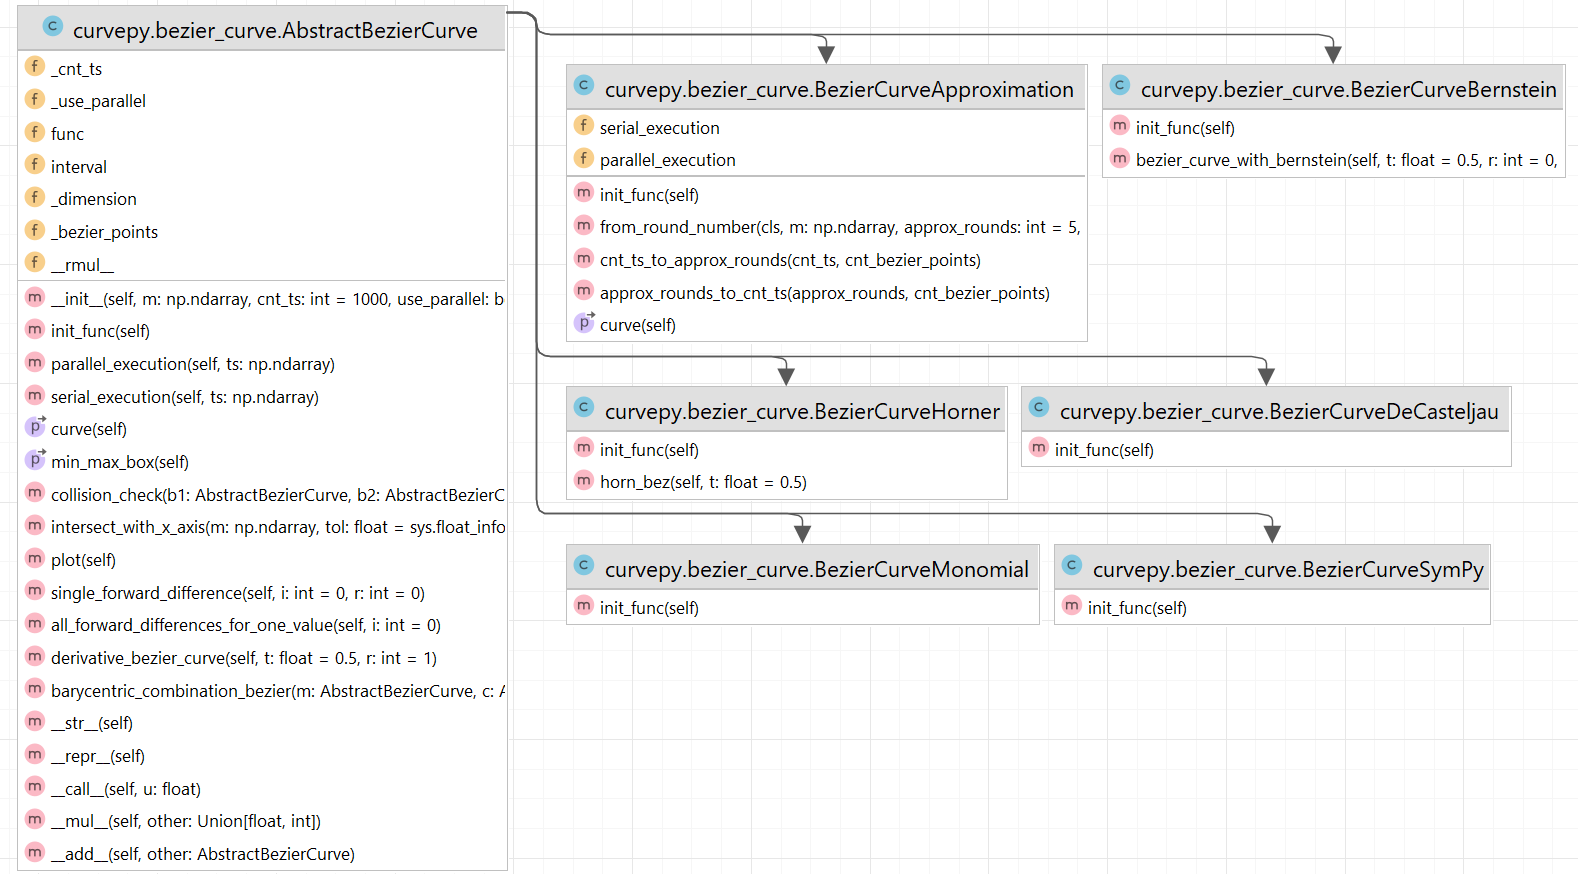
\includegraphics[width=\textwidth]{uml.png}
    \caption{UML class diagram of all Bézier curves}
    \label{fig:my_label}
\end{figure}
\newpage
\subsection{De-Casteljau Algorithm}
In this section we will first introduce the De-Casteljau algorithm which can calculate points lying on a Bézier curve. Following that we explain some interesting properties of Bézier curves and then present our different implementations.

\begin{definition}
Let $b_0, \dots, b_n \in \mathbb{R}^2$ and $t \in \mathbb{R}$, then the following formula is used for the \textbf{De-Casteljau} algorithm:
\[b_i^r(t) = (1-t) \cdot b_i^{r-1}(t) + t \cdot b_{i+1}^{r-1}(t)\]
for $r = 1, \dots, n$ and $i = 0, \dots, n-r$. \\
\end{definition}
\subsubsection{Endpoint Interpolation}
If $t$ is set to $0$ we get $b_0$ (i.e. the beginning) and if it is set to $1$ we get $b_n$ (i.e. the end), which allows for easier usage, especially in design-oriented problems. This is also very handy for composing Bézier curves.

\subsubsection{Invariance under Affine Maps}
Bézier curves are invariant under affine maps, which follows from the De-Casteljau algorithm, since it uses repeated linear interpolation, which is invariant under affine maps. This property is quite handy. For instance if we have four control points and want to evaluate 100 points on the curve described by them and additionally we want to rotate these points, we can just rotate the control points and then compute the 100 points instead of first computing all 100 points and then rotating everyone of them.

\subsubsection{Parameter Transformation}
Another interesting property is that the curve is blind to the actual interval, that the curve is defined over. This is possible, because the algorithm works on ratios. Furthermore we can map a parameter $u$ from an arbitrarily chosen interval $[a,b]$ on our unit interval $[0,1]$ by applying the following transformation: \[t = \frac{u-1}{b-a}\]

\subsubsection{Blossoms and De-Casteljau}
The concept of blossoming can also be used in the De-Casteljau algorithm. One can use a new parameter value $t \in [0,1]$ in each step of the algorithm. Looking at the cubic case we obtain:
\begin{center}
  \begin{tabular}{ l c r r}
  $b_0$ &         \\
  $b_1$ & $b_0^1[t_1]$ &      \\
  $b_2$ & $b_1^1[t_1]$ & $b_0^2[t_1, t_2]$    \\
  $b_3$ & $b_2^1[t_1]$ & $b_1^2[t_1, t_2]$ & $b_0^3[t_1, t_2, t_3]$\\
\end{tabular}
\\
\end{center}
This traces out a region because we use in each of our $r$ steps a different value $t_r$, to recover the original point on the curve we need to set $t = t_1 = t_2 = t_3$ and compute again. 

\subsubsection{Implementation}
We divided the De-Casteljau algorithm in three methods:
\begin{enumerate}
    \item[1] \texttt{de\_casteljau\_one\_step}. This method computes one step of the De-Casteljau algorithm using the following formula:
    \[b_i^r(t) = (1-t) \cdot b_i^{r-1}(t) + t \cdot b_{i+1}^{r-1}(t)\]
    Because of numpy arrays the implementation is straightforward. We utilise slicing and element wise operations on numpy arrays to compute one step without the use of a loop. Additionally we perform most of the heavy work in C++, which makes our implementation significantly faster than only using Python.
    \item[2] \texttt{de\_casteljau\_n\_steps}. This method calls (1) $n$ times, where $n$ lies between \texttt{0} and number of control points minus one and is given by the user. So one can calculate intermediate points or resume calculation from intermediate points.
    \item[3] \texttt{de\_casteljau}: This method computes $b_0^n(t)$ by calling (2) with the proper value for $n$, which is the number of control points minus one.
\end{enumerate}
One drawback is, that we have to explicitly copy the array in certain steps to avoid mistakes, since all python objects, including numpy arrays, are called by reference. We also implemented a parallel version of (3). \\

\begin{figure}[H]
    \centering
    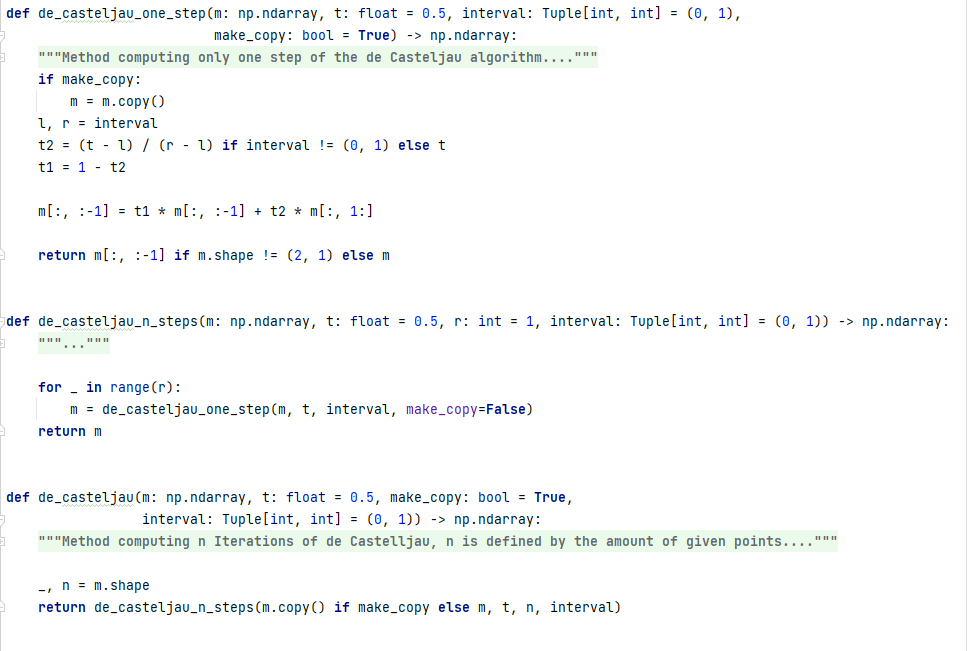
\includegraphics[width=\textwidth]{de_cas.png}
    \caption{De-Casteljau Code}
    \label{fig:my_label}
\end{figure}

There is also a sympy version of the De-Casteljau algorithm, which handels $t$ as a symbolic variable and computes the algorithm without knowing a specific value for $t$, hence we end up with a function representing our curve. At the end we use the lambdify routine to transform our symbolic function to a lambda function, so that we can calculate numerical values faster. Thus for every value of $t$ we just evaluate our lambda function for this value. Sadly, this implementation is limited by the maximum recursion depth allowed by Python.\\

Our blossoming method calls \texttt{de\_casteljau\_one\_step} for different values of $t$ which are defined by the user in a given list.
\newpage
\subsection{Bernstein}
Another way to calculate Bézier curves is to use Bernstein polynomials.
We define them as follows.
\begin{definition}
For $t \in \mathbb{R}$ we define:
\[B_i^n(t) = \binom{n}{i} \cdot t^{i} \cdot (1-t)^{n-i}\]
as the \textbf{Bernstein Polynomial} with parameter $t$, where
\[
\binom{n}{i} =
\left\{
	\begin{array}{ll}
		\frac{n!}{i! \cdot (n-i)!}  & \mbox{: } 0 \leq i \leq n \\
		 0 & \mbox{: } otherwise
	\end{array}
\right.\]
\end{definition}
There is also a recursive formula for Bernstein polynomials:
\begin{definition}
The \textbf{Bernstein polynomial} with parameter $t$ is defined as follows:
\[B_i^n(t) = (1-t) \cdot B_i^{n-i}(t) + t \cdot B_{i-1}^{n-1}(t)\]
where $B_0^0(t)=1$ and $B_j^n(t)=0$ for $j \notin \{0, \dots, n\}$.\\
\end{definition}
We implemented both the recursive and the iterative variant.
\begin{rem}
From the blossoming section we know that we can write Bézier curve as $b[t^n]$, moreover $t$ can be expressed as $t=(1-t) \cdot 0 + t \cdot 1$. By applying \cref{leib} we get
\[b(t) = b[t^n] = \sum_{i=0}^n b_i \cdot B_i^n(t)\]
since $b_i = b[0^{n-i}, 1^{i}]$.
\end{rem}
This results in the following remark:
\begin{rem}
We can express the intermediate points $b_i^r$ in the form of Bernstein polynomials of degree $r$:
\[b_i^r = \sum_{j=0}^r b_{i+j} \cdot B_j^r(t)\]
This follows because of $b_i^r(t) = b[0^{n-r-i}, t^r, 1^{i}]$ and \cref{leib}.
\end{rem}

With this at our hands we get:
\begin{theorem}
Given control points $b_0, \dots, b_n \in \mathbb{R}^2$ and a parameter $t \in [0,1]$. Further let $b_i^r, i \in \{1, \dots, n\}, r < n$ be precomputed. Then we can extend our $b^r$ values as follows:
\[b^n(t) = \sum_{i=0}^{n-r} b_i^r(t) \cdot B_i^{n-r}(t)\]
\end{theorem}

This means that $r$ semantically describes the highest degree of the previously computed Bézier polygon. Thus $r=0$ if and only if no precomputation was made beforehand.\\

Additionally we have the property of invariance under barycentric combinations:
\[\sum_{i=0}^n (\alpha \cdot b_i + \beta \cdot c_i) \cdot B_i^n(t) = \sum_{i=0}^n \alpha \cdot b_i \cdot B_i^n(t) + \sum_{i=0}^n \beta \cdot c_i \cdot B_i^n(t)\]

Therefore we implemented two magic methods namely the \texttt{\_\_add\_\_} and \texttt{\_\_mul\_\_} function. \texttt{\_\_add\_\_} just adds up the given Bézier points of both curves and \texttt{\_\_mul\_\_} multiplies all control points by a scalar value.

\begin{figure}[H]
    \centering
    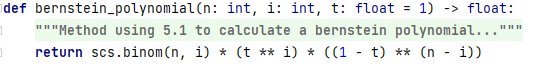
\includegraphics[width=\textwidth]{bernstein_polynomial.png}
    \caption{Bernstein Polynomial Code}
    \label{fig:my_label}
    \centering
    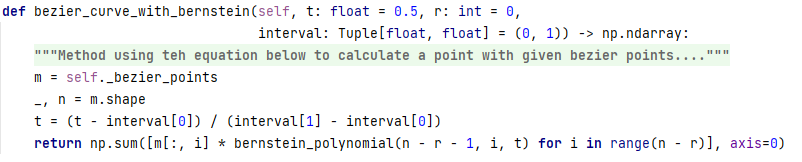
\includegraphics[width=\textwidth]{bernstein.png}
    \caption{Bézier with Bernstein Code}
    \label{fig:my_label}
\end{figure}
\newpage
\subsection{Horner Scheme}
We can also develop an Horner Scheme for the Bézier curves. First we will look at a cubic example.
\begin{example}
\[c_0 + t \cdot c_1 + t^2 \cdot c_2 + t^3 \cdot c_3 = c_0 + t \cdot (c_1 + t \cdot (c_2 + t \cdot c_3))\]

This is the case for a normal polygon on the monomial base, where $c_0, \dots, c_4 \in \mathbb{R}$ and $t \in \mathbb{R}$. We can transform this to Bézier curves and get
\[b^3(t) = \left(\left(\binom{3}{0} \cdot s \cdot b_0 + \binom{3}{1} \cdot t \cdot b_1\right) \cdot s + \binom{3}{2} \cdot t^2 \cdot b_2\right) \cdot s + \binom{3}{3} \cdot t^3 \cdot b_3\]
where $s = (1-t)$, with $t \in \mathbb{R}$ and $b_0, \dots, b_3 \in \mathbb{R}^2$.
\end{example}
Now we can generalize this in the following way:
\begin{definition}
Given $n \in \mathbb{N}$ points $b_0, \dots, b_n \in \mathbb{R}^2$ and a parameter $t \in \mathbb{R}$ we can describe $b^n(t)$ in the following way:
\[b^n(t) = \left(\dots\left(\left(\left(\binom{n}{0} \cdot s \cdot b_0 + \binom{n}{1} \cdot t \cdot b_1\right) \cdot s + \binom{n}{2} \cdot t^2 \cdot b_2\right) \cdot s + \binom{n}{3} \cdot t^3 \cdot b_3\right) \dots\right) \cdot s + \binom{n}{n} \cdot t^n \cdot b_n\]
where $s = (1-t)$. \\
\end{definition}
This method is faster than the normal De-Casteljau algorithm, since the Horner scheme is of order $\mathcal{O}(n)$ while De-Casteljau is of order $\mathcal{O}(n^2)$. Additionally we do not need to save the control polygon in auxiliary array which saves space and further boosts the performance.
\begin{figure}[H]
    \centering
    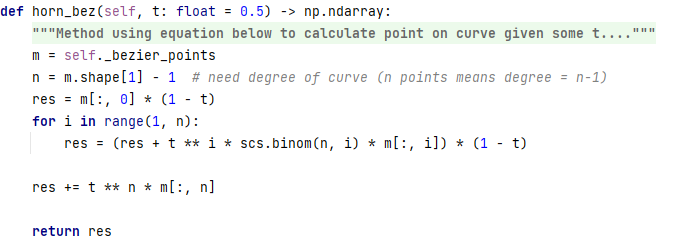
\includegraphics[width=\textwidth]{horner.png}
    \caption{Bézier with Horner Scheme Code}
    \label{fig:my_label}
\end{figure}
Note that \texttt{m} is just a reference to the control polygon for simplicity's sake.

\subsection{Monomial Form of Bézier Curve}
Before we start with the monomial form we need to know how to calculate the derivatives of Bézier curves.
\begin{definition}\label{diff}(Forward Differences and Iterated Forward Differences)
Given some points $b_0, \dots, b_n$ over $\mathbb{R}^2$.
The \textbf{forward difference} is defined as follows:
\[\Delta b_j = b_{j+1} - b_j\]
We can go one step further and define the \textbf{iterative forward differences}:
\[\Delta^r b_i = \sum_{j=0}^r \binom{n}{j} \cdot (-1)^{r-j} \cdot b_{i+j}\]
\end{definition}
These will become handy when we inspect the derivatives and the monomial form.
\newpage
\subsubsection{Derivative of Bézier Curves}
Before we will have a look at the general derivative, let us first examine the first derivative.
\begin{theorem}
For the first \textbf{derivative} we first compute one step of De-Casteljau with $t=1$ and then with an arbitrary $t \in [0,1]$ the next $n-1$ steps.
\[b^\prime(t) = n \cdot \sum_{j=0}^{n-1} \Delta b_j B_j^{n-1}(t)\]
Alternatively we can perform $n-1$ steps of De-Casteljau with respect to some $t \in [0,1]$ and then exactly one step with $t=1$.
\[b^\prime(t) = n \cdot (b_1^{n-1}(t) - b_0^{n-1}(t))\]
\end{theorem}
This leads to an interesting property.
\begin{rem}
The derivative of a Bézier curve is just another Bézier curve, hence the derivative is a byproduct of the De-Casteljau algorithm. Though the De-Casteljau algorithm is not the fastest way of computing a Bézier curve, it is useful whenever we also need the first derivative.
\end{rem}
With the help of \cref{diff} we get a formula for the $r$'th derivative.
\begin{theorem}\label{deriv}
For a Bézier curve described by $b_0, \dots, b_n \in \mathbb{R}^2$ we get that the $r$th derivative is described by
\[\frac{d^r}{dt^r}b^n(t) = \frac{n!}{(n-r)!} \cdot \sum_{j=0}^{n-r} \Delta^r b_j \cdot B_j^{n-r}(t)\]
where $\Delta^r b_j$ is the iterated forward difference of $b_j$ for $j \in \{1, \dots, n\}$.
\end{theorem}
Since we can know easily compute the derivatives we can generate the Taylor series, which is our monomial form, since we are in the polynomial case.
\[x(t) = \sum_{j=0}^n \frac{1}{j!} \cdot x^{(j)}(0) \cdot t^j \]
When we use \cref{deriv} we get:
\newpage
\begin{theorem}
The monomial Form of a Bézier curve with the control points $b_0, \dots b_n \in \mathbb{R}^2$ is decribed by the formula
\[b^n(t) = \sum_{j=0}^n \binom{n}{j} \cdot \Delta^j b_0 \cdot t^j\]
where $\Delta^j b_0$ is the iterated forward difference of $b_0$.
\end{theorem}

\subsubsection{Implementation}
We again use sympy to first calculate the polynom as a symbolic function. This is done by computing the coefficient $\binom{n}{j} \cdot \Delta^j b_0$ and multiplying it with the symbol $t^j$. Finally we use lambdify to fasten up the computation of the function. Hence we end up with a lambda function which takes a $t$ as input and calculates the point. Alternatively one could use the presented Horner scheme by first constructing a list of the coefficients, that has to be done just once, and after that just call the method with the list and every value for $t$.\\

However this form is \textbf{numerical very unstable} and should be avoided whenever possible.

\subsection{Subdivision}
Let us turn our attention to a different approach of computing Bézier curves.
\begin{definition}(Subdivision)
Given $b_0, \dots, b_n \in \mathbb{R}^2$ we run the De-Casteljau algorithm for some given parameter $t \in \mathbb{R}$. After that, we divide our set of points into two. First set is over the interval $[0,t]$, we will denote this points $l_0, \dots, l_n \in \mathbb{R}^2$. The second set is over the interval $[t,1]$, we call these points $r_0, \dots, r_n \in \mathbb{R}^2$. We repeat this procedure for some given amount of $k \in \mathbb{N}$ rounds.
\end{definition}
So subdivision can be seen as an \textbf{approximation} of the curve described by our initial Bézier polygon since we get $2\cdot(n+1)$ points per iteration, which can again be subdivided. Obviously, the more points we evaluate, the better the approximation becomes.
\begin{rem}
After $k \in \mathbb{N}$ rounds of subdivision, one gets $2^k$ Bézier polygons with $n+1$ points each.
\end{rem}
This can easily be seen as per round of subdivision we get two sets of points and we apply subdivision on them in the next step. This leads to a relatively fast approximation of our Bézier curve.
\begin{example}
After $10$ rounds of subdivision with $b_0, \dots, b_5 \in \mathbb{R}^2$ we get $1024$ Bézier polygons each consisting of $6$ points.
\end{example}
Now we will have a look at which points one should pick for the left and right set of points.
\begin{example}
If we look at the cubic example it is also easy to see which points to pick.
\begin{center}
  \begin{tabular}{ l c r r}
  \textcolor{red}{$b_0$} &         \\
  $b_1$ & \textcolor{red}{$b_0^1$} &      \\
  $b_2$ & $b_1^1$ & \textcolor{red}{$b_0^2$}    \\
 \textcolor{blue}{$b_3$} & \textcolor{blue}{$b_2^1$} & \textcolor{blue}{$b_1^2$} & \textcolor{Plum}{$b_0^3$}\\
\end{tabular}
\\
\end{center}

We just take the \textcolor{red}{hypotenuse} and the \textcolor{blue}{bottom line} of the scheme. However the bottom line is taken in \textbf{reversed} order and not from left to right.
\begin{figure}[H]
    \centering
    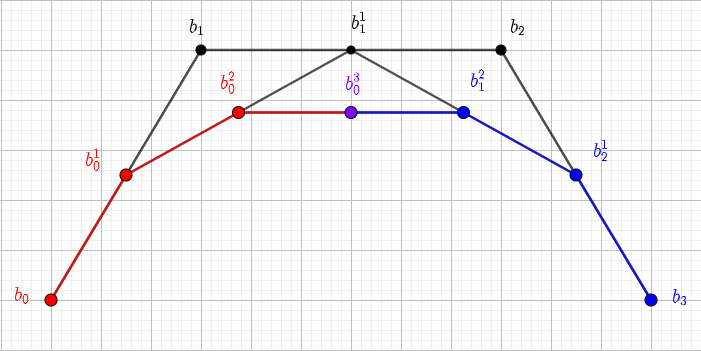
\includegraphics[width=\textwidth]{SubdivisionExamplePic.PNG}
    \caption{Subdivision Example with $t=0,5$}
    \label{fig:my_label}
\end{figure}
In the end we get two new Bézier polygons, which both have four points like the one we had in the beginning, the left one in red with the points $b_0$, $b^1_0$, $b^2_0$ and $b^3_0$ which is shared with the blue Bézier polygon on the right, consisting of $b^3_0$, $b^2_1$, $b^1_2$ and $b_3$.
\end{example}


\subsubsection{Implementation}
We implemented the described procedure in the following way. The \texttt{current} variable represents one column of the triangular scheme we presented. By setting the $ith$ element of \texttt{left} to the fist element of \texttt{current} in every step we always ensure that only elements lying on the hypotenuse are saved in \texttt{left}. The array \texttt{right} works in a quite similar manner but as we want the reverse order we begin at the end of the array and always look at the last element of current which is an element from the bottom line of the scheme. At last in every iteration we call \texttt{de\_casteljau\_one\_step} which returns the next column saved in \texttt{current}. 

\begin{figure}[H]
    \centering
    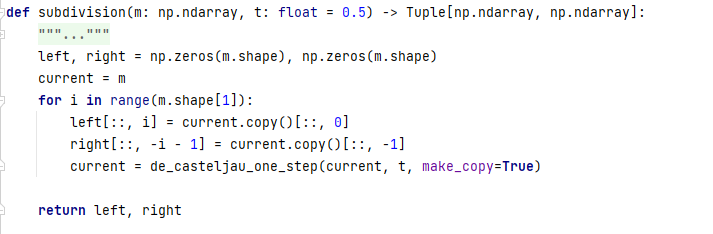
\includegraphics[width=\textwidth]{subdivision.png}
    \caption{Subdivision Code}
    \label{fig:my_label}
\end{figure}

This implmenentation differs a bit; since we double the number of points each time, we have to compute the number of rounds needed for the expected accuracy. We use the following formula:
\[approx\_rounds = \ceil[\bigg]{\log_2 \frac{|\text{points to be calculated}|}{|\text{bezier points}|}}\]
\begin{figure}[H]
    \centering
    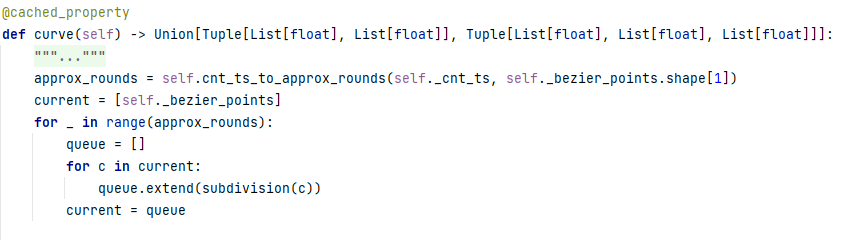
\includegraphics[width=\textwidth]{subdiv_approx_curve.png}
    \caption{Subdivision Code}
    \label{fig:my_label}
\end{figure}
\newpage
With \texttt{approx\_rounds} determined we start a nested loop in which we subdivide for each array contained in \texttt{current}. The resulting \texttt{left} and \texttt{right} are saved in \texttt{queue} which is a temporary storage. At the end we overwrite \texttt{current} with \texttt{queue}. This is done \texttt{approx\_round} times. So for each \texttt{c} in \texttt{current} we get two new arrays. This results in the $2^k$ Bézier polygons where $k$ equals \texttt{approx\_rounds}.

\subsection{Intersection}
In this last section we do not explain another calculation method but instead how one can check whether two Bézier curves intersect thanks to two concepts.

\subsubsection{MinMaxBox}
The MinMaxBox, which is the smallest axis parallel box containing all control points, uses the property of the convex hull. Since all intermediate points $b_i^r$ are computed by a convex barycentric combination of previous points, we never get points outside the convex hull of the $b_i$. Therefore the hole curve described by the control polygon lies within the convex hull. So when we want to perform a fast check of intersection we can construct the MinMaxBox of the two curves, which is just a box containing the control polygon and therefore the curve itself as well. To check if these two boxes intersect can easily be done. If we get a false we can return \texttt{False}. In the other case we have to be more precise. However we can very fast determine if two curves could intersect, which is pretty useful, because we maybe want to check the intersection of multiple curves and with the help of these boxes we can maybe eliminate some curves without taking much effort. 
\subsubsection{Approximate Intersection}
If the two boxes indicate an intersection we have to be more precise, since the intersection of boxes is very coarse. In this case we use subdivision. We split our original curve into sub polygons and check for these ones if their boxes intersect or not, one might call this "divide and conquer". If they do not intersect we can return \texttt{False}. However if they intersect and the areas of the boxes are very small (is defined by a tolerance parameter), we can return \texttt{True}, because our boxes intersect and the box itself can be seen as the part of the curve we are looking at. This is reasonable as we are inherently limited by the floating point precision.\\

In the other cases we just split up again. At the end we check if one of our calls has returned $True$, because then we can say, that the curves intersect with some given tolerance.
\begin{figure}[H]
    \centering
    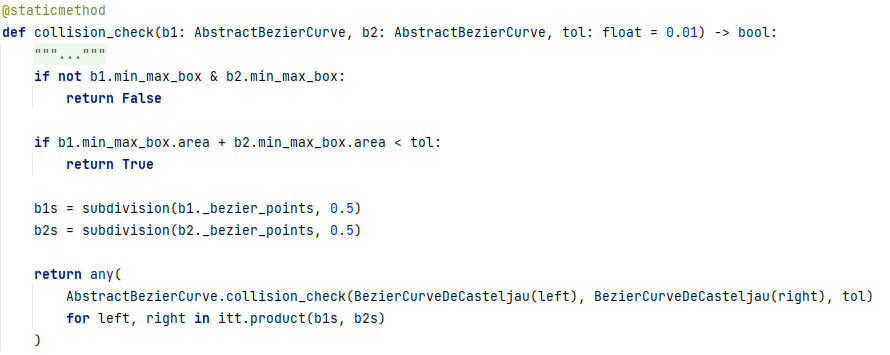
\includegraphics[width=\textwidth]{collision_check.png}
    \caption{Approximate Intersection Code}
    \label{fig:my_label}
\end{figure}

\subsection{Benchmarks}
In order to compare the different algorithms for computing Bézier curves, we ran benchmarks using the same control points.
\subsubsection{Benchmark Configuration}
We used the following configuration:
\begin{itemize}
    \item Dell OptiPlex 5090 Micro
    \item 11th Gen Intel(R) Core(TM) i5-11500T @ 1.50GHz
    \item 1x16 GB non-ECC DDR4 RAM
    \item 256GB NVME M.2 SSD
    \item Ubuntu 20.04.4 LTS (deployed via PXE)
    \item Python 3.8.10
\end{itemize}
The PC was completely idling while running the benchmarks; the idle CPU workload was significantly below 1\%.

\subsubsection{Results}
At first, we compared all viable Bézier curves with each other:
\begin{figure}[H]
    \centering
    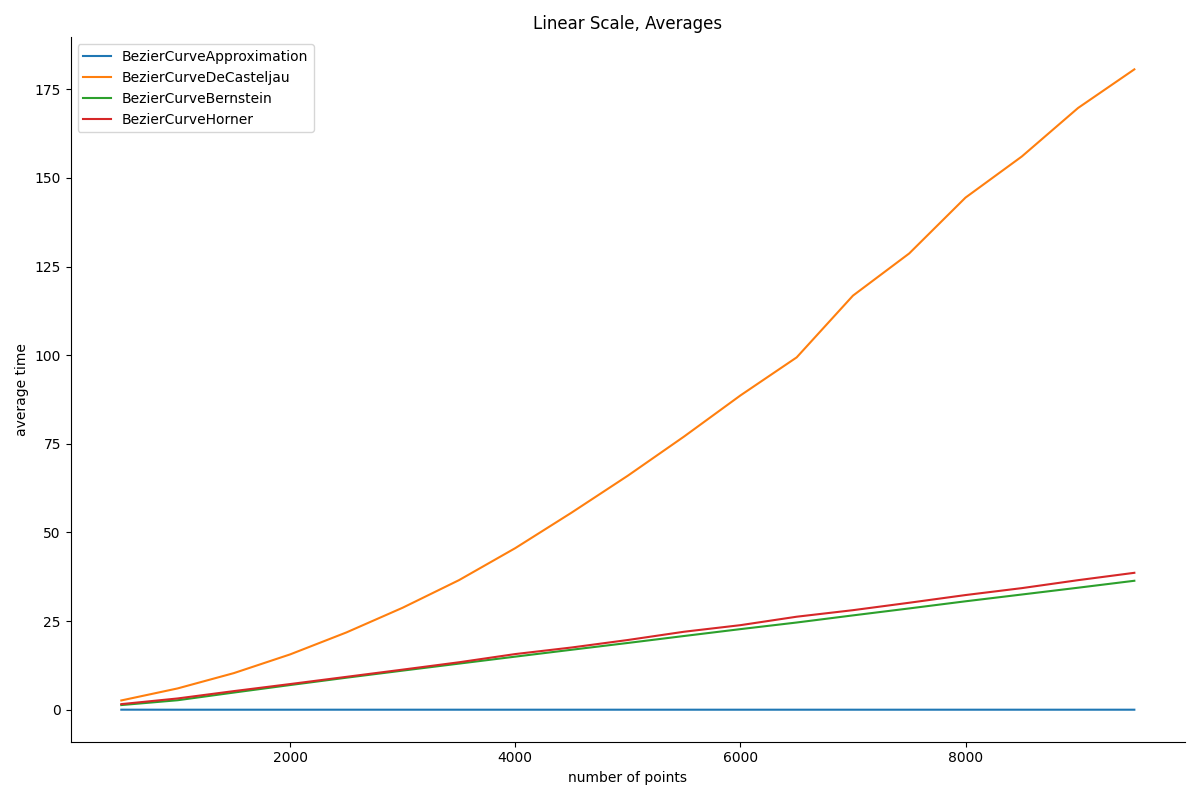
\includegraphics[width=0.9\textwidth]{bezier_lin.png}
    \caption{Average runtime in s}
    \label{fig:my_label}
\end{figure}
To make it more readable, let's look at a logarithmic y-axis:
\begin{figure}[H]
    \centering
    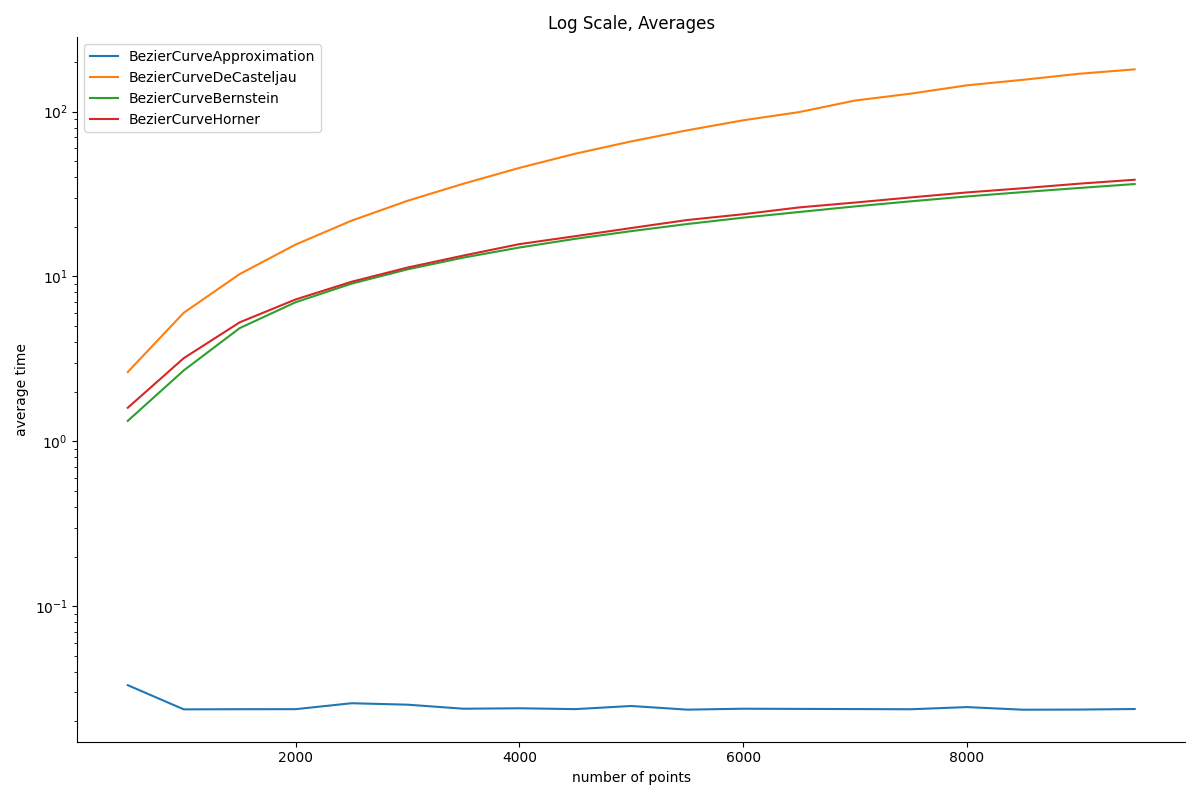
\includegraphics[width=0.9\textwidth]{bezier_log.png}
    \caption{Average runtime in s; logarithmic scale}
    \label{fig:my_label}
\end{figure}
The approximation algorithm seems to have constant runtime. This is not true; as we increase the problem size the real complexity emerges:
\begin{figure}[H]
    \centering
    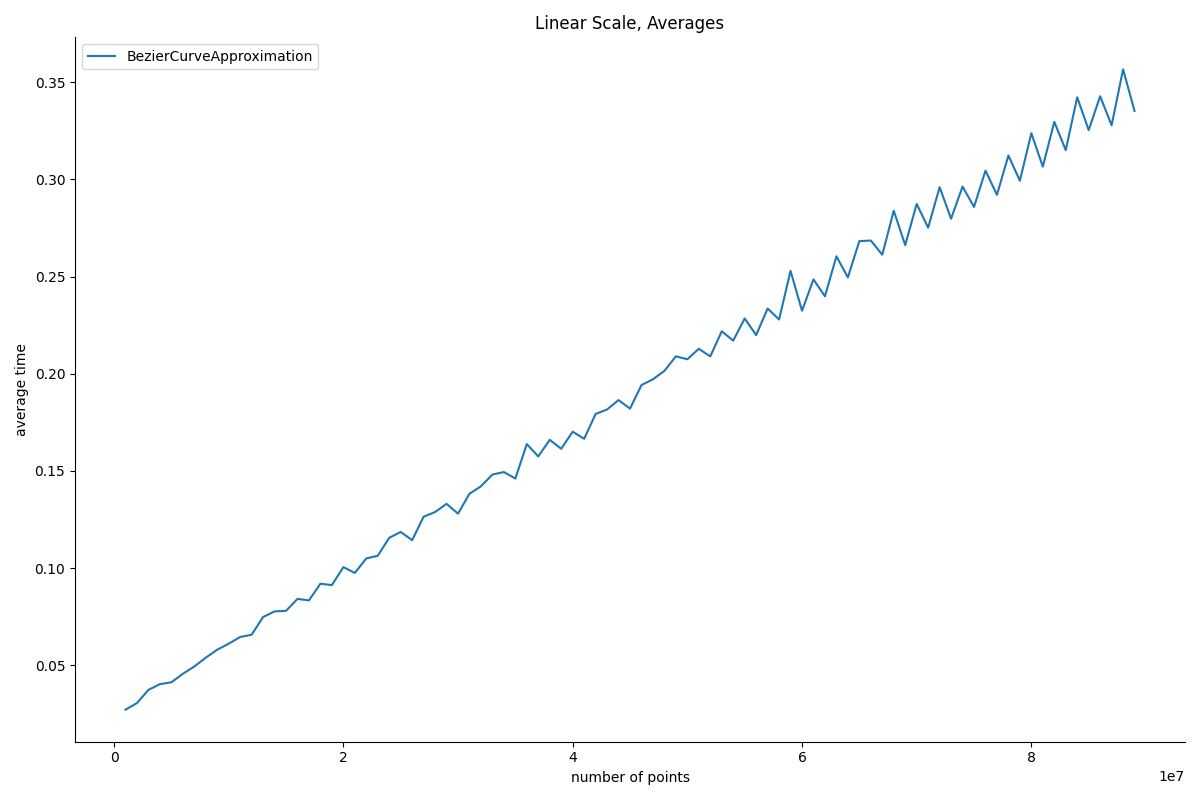
\includegraphics[width=0.9\textwidth]{Approx_lin.png}
    \caption{Average runtime in s}
    \label{fig:my_label}
\end{figure}
Again, in logarithmic scale:
\begin{figure}[H]
    \centering
    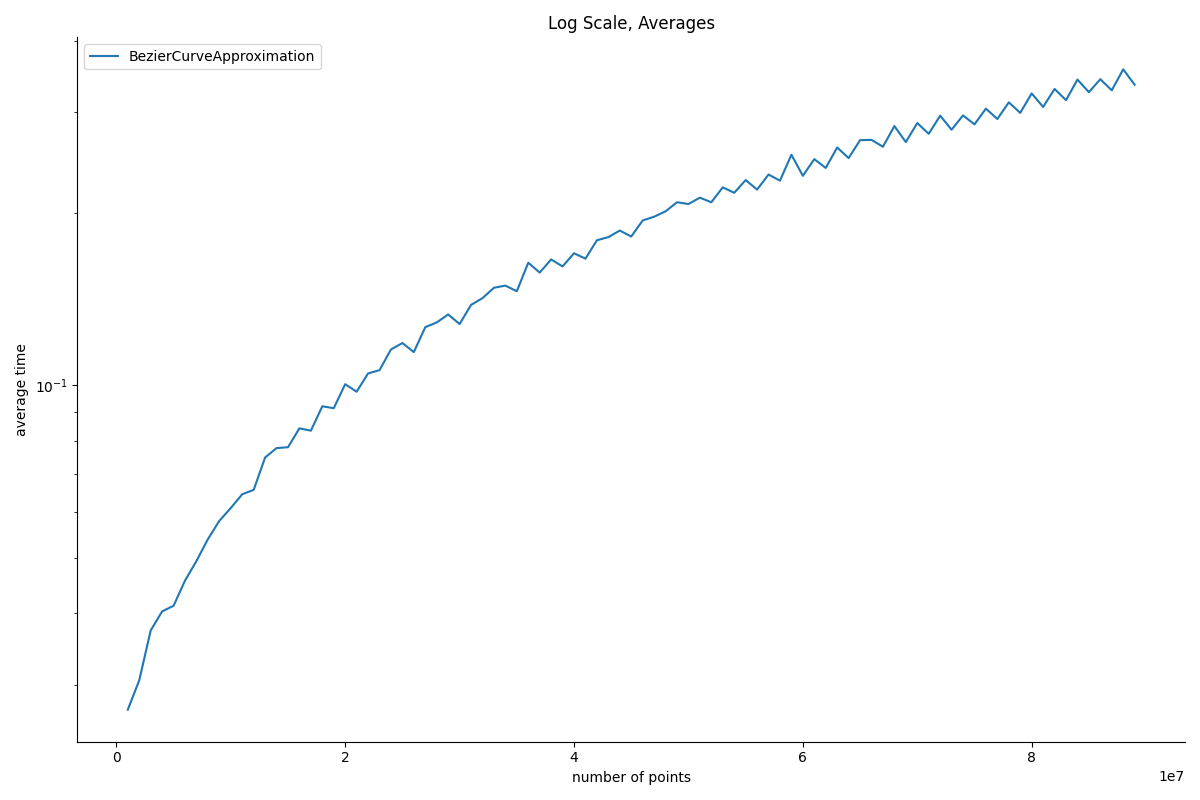
\includegraphics[width=0.9\textwidth]{Approx_log.png}
    \caption{Average runtime in s; logarithmic scale}
    \label{fig:my_label}
\end{figure}
Those are great results, since the computed Bézier curve is, from a visual perspective, basically indistinguishable.
\begin{figure}[H]
\centering
\begin{subfigure}{.5\textwidth}
  \centering
  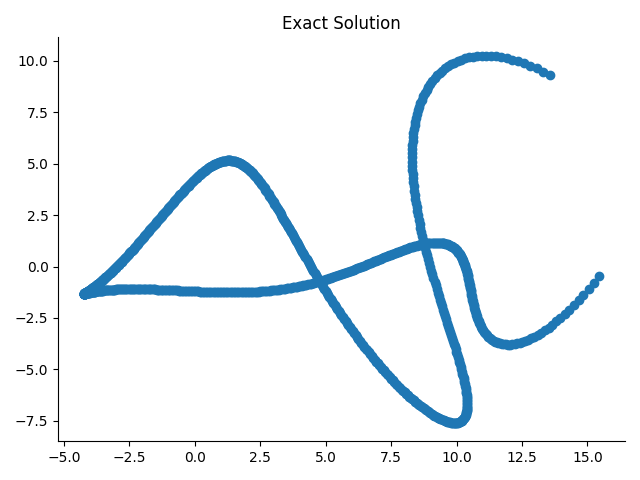
\includegraphics[width=\linewidth]{Comp_Exact.png}
\end{subfigure}%
\begin{subfigure}{.5\textwidth}
  \centering
  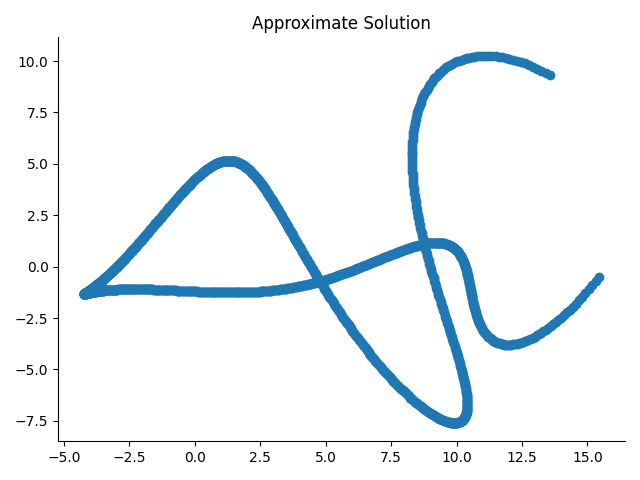
\includegraphics[width=\linewidth]{Comp_Approx.png}
\end{subfigure}
\caption{Both algorithms resulting in the approximately same curve}
\label{fig:test}
\end{figure}

\subsubsection{Problems}
While benchmarking, we encountered two problems:
\begin{enumerate}
    \item As mentioned in the literature \cite{10.5555/501891}, the monomial algorithm is very badly conditioned. Thus, the problem is numerically instable. This would usually not be a problem as Python supports dynamically sized integers. But for large numbers, any floating point values will overflow as they comply with the IEE754 floating point standard. Since $t \in [0,1]$, this can't be avoided.
    \item The Sympy solution does not work for large numbers. This has a rather practical reason. For historical design reasons, Python is designed in such a way that it does not, and will never, support tail call optimization. Therefore the stack space increases linearly with the recursion depth. In order to not get terminated by a segmentation error, Python limits the recursion depth by the variable \texttt{sys.setrecursionlimit}. This also limits the solvable problem size of our Sympy based solution.
\end{enumerate}
\newpage
\section[Voronoi and Delaunay]{Voronoi Regions, Dirichlet Tessellations and Delaunay Triangulations}
\subsection{Motivation}
Given an arbitrary set of points in the 2D plane, a \textit{Voronoi Diagram} or \textit{Dirichlet Tessellation} divides the plane into tiles; each point is associated with the region of the plane closest to it.\\~\\
\begin{figure}[H]
    \centering
    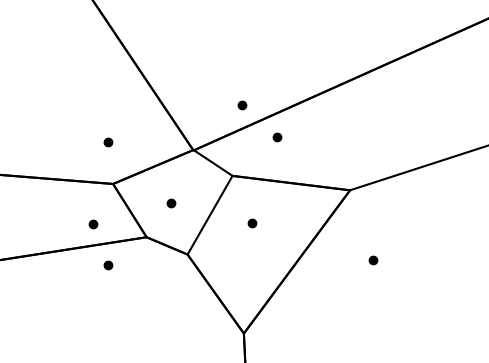
\includegraphics[width=0.7\textwidth]{voronoi.png}
    \caption{Points and their Voronoi regions}
    \label{fig:my_label}
\end{figure}
Voronoi diagrams are of monumental importance in many different branches of science and were rediscovered numerous times. Geographers speak of Thiessen polygons, which are used as models for crystal growth, while Metallurgists speak of Wigner-Seitz zones for analyzing equilibrium properties of alloys. As we see later, its dual graph, the \textit{Delaunay Triangulation}, also has various applications in other fields, for example as an automatic mesh generator used in finite element methods. Voronoi Diagrams are especially useful for many problems in the field of computational geometry.
\newpage
\cite{Aurenhammer1991} summarizes the importance as follows:
\begin{quote}
    Accordingly, Voronoi diagrams are useful in three respects: As a structure per se that makes explicit natural processes, as an auxiliary structure for investigating and calculating related mathematical objects, and as a data structure for algorithmic problems that are inherently geometric.
\end{quote}
For a more exhaustive list of applications, see \cite{Aurenhammer1991}.
\subsection{Definitions and Theorems}
We use the formal definitions provided by \cite{Green1978}.
\begin{definition}[Voronoi tile]
Let $\mathcal{P}_N := \{P_1, P_2, \dots, P_N\}$ be finitely many points in the plane such that $P_i \neq P_j, i\neq j$. The \textbf{Voronoi tile} of $P_i$ is the set $T_i$ defined by
\[
T_i = \{
  x : d(x, P_i) < d(x, P_j), \forall j \neq i
\}
\]
where $d$ is the euclidean distance.
\end{definition}
Note that tiles are infinite if and only if they are not entirely surrounded by other tiles. Further note that all tiles are trivially convex.\\
Not every point is part of a tile. Let $P_n$ and $P_m$ be 2 points and $T_n$, $T_m$ be their neighbouring tiles. If $x$ is a point such that $d(x, P_n) = d(x, P_m)$ then $x$ lies in neither $T_n$ nor $T_m$. This is why tiles are open, all points neighbouring 2 or more tile centers form the \textbf{boundary segments} of that tile.
\begin{definition}[Voronoi Diagram, Dirichlet Tessellations]
A \textbf{Voronoi Diagram}, also called a \textbf{Dirichlet Tessellation}, is the set of all tiles and boundaries subdividing a given space.
\end{definition}
Although intuitively understandable, let us formally define what a neighbour is:
\begin{definition}[Neighbour]
Two Voronoi Tiles are \textbf{neighbours} if and only if they share one boundary segment.
\end{definition}
Through Voronoi diagrams, we can easily get another important geometric structure.
\begin{definition}[Triangulation]
A \textbf{triangulation} is a subdivision of an object into simplicies. Note that in 2D, this is a subdivision into triangles.
\end{definition}
\begin{definition}[Delaunay Triangulation]
Let $\mathcal{P}_N$ be finitely many points in the plane, no two of which coincide. Further let $T_1, \dots, T_n$ be the Voronoi tiles of those points. The \textbf{Delaunay Triangulation} is a triangulation of these points with the following property:
\[
\forall i,j \in \{1,\dots,n\}, i \neq j: (P_i, P_j) \text{ are connected } \Leftrightarrow (T_i, T_j) \text{ are neighbours }
\]
This makes the Delaunay Triangulation the \textbf{dual graph} of the Voronoi Diagram (See \cite{FORTUNE1995}, Theorem 2.1.3)
\end{definition}
\begin{figure}[H]
    \centering
    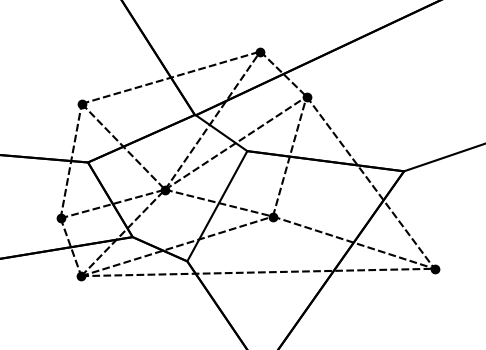
\includegraphics[width=0.7\textwidth]{delaunay.png}
    \caption{Voronoi Regions and Delaunay triangulations as it's dual graph}
    \label{fig:my_label}
\end{figure}
The Delaunay Triangulation has a few useful properties, a few of which we list here. For a more in depth discussion, see \cite{Aurenhammer1991}.
\begin{theorem}[Existance of a Delaunay Triangulation]
Let $\mathcal{P}_N$ be finitely many points. If the euclidian metric is used, a Delaunay triangulation always exists.
\end{theorem}
This follows from the definition of the Voronoi diagram, which always exists.
\begin{theorem}[Circumcircle property]
For any Delaunay triangulation, the circumcircle of any triangle does precisely only contain the 3 points defining the triangle.
\end{theorem}
Note that this theorem was used by Delaunay as the triangulation definition \cite{Aurenhammer1991}.
\begin{figure}[H]
    \centering
    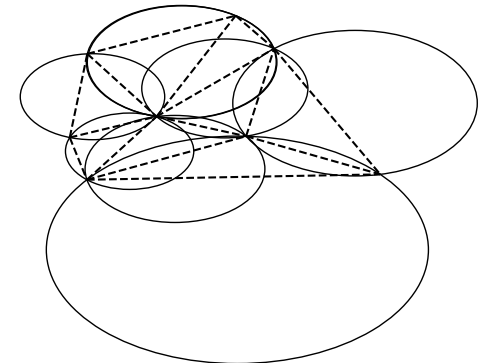
\includegraphics[width=0.7\textwidth]{circumcircle.png}
    \caption{Delaunay triangulations and their Circumcircles}
    \label{fig:my_label}
\end{figure}
\begin{theorem}[Optimality]
Over all proper $2D$ triangulations, the Delaunay triangulation maximizes the minimum angle of any triangle.
\end{theorem}
\begin{proof}
See \cite{FORTUNE1995} Theorem 3.1
\end{proof}
This implies that the Delaunay triangulation is the most equiangular one, which makes it computationally more desirable in finite element and interpolation methods \cite{Aurenhammer1991} \cite{Rebay1993}.
\subsection{Possible Algorithms}
Here follows a short overview on different types on algorithms. For convenience reasons we will present all algorithms in terms of the Delaunay triangulation instead of the Voronoi diagram, which is easily obtained from any graph-based Delaunay representation. For a more detailed discussion, see \cite{FORTUNE1995}.\\
The following bounds are known for computing Delaunay triangulations \cite{FORTUNE1995}:
\begin{itemize}
    \item For $2$ dimensional Delaunay triangulations, a worst case lower bound of $\Omega(n \log n)$ is known.
    \item For $d > 2$ dimensional Delaunay triangulations, an lower bound of $\Omega(n^{\lceil d/2 \rceil})$ is known.
\end{itemize}
\subsubsection{Flip Algorithm}
Flipping algorithms are the most simple type of algorithm. At first, you start with some kind of triangulation, which doesn't have any further constraints. From there on, we can just "flip" edges until every edge furfills the circumcircle property. The mapping from the starting triangulation to the ending one is called a \textbf{transformation}. Formally:
\begin{theorem}[flips and flippable edges]
Let $\Delta_1, \Delta_2$ be two neighbouring triangles with $e$ being the edge contained in both boundaries. If the union of both triangles $C := \Delta_1 \cup \Delta_2$ forms a convex quadrilateral, $e$ is \textbf{flippable}. \textbf{Flipping} $e$ means replacing $e$ with it's diagonal in $C$.
\end{theorem}
\begin{figure}[H]
    \centering
    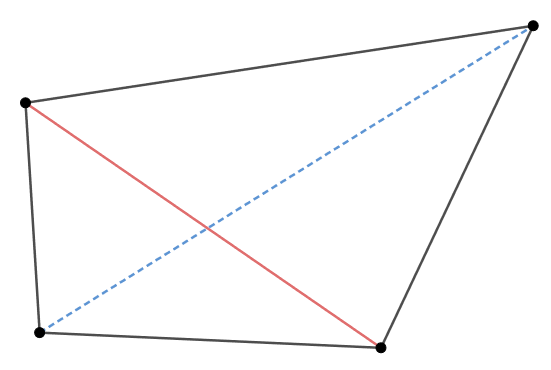
\includegraphics[width=0.7\textwidth]{flippable.png}
    \caption{A flippable edge (red), it's alternative (blue) and the required convex quadrilateral (black)}
    \label{fig:my_label}
\end{figure}
While this class of algorithms is conceptually very simple, it has very poor performance, with some transformations requiring at least $\Omega(n^2)$ flips \cite{Hurtado1999}.
\subsubsection{Incremental Algorithm}
The incremental algorithm works by using the circumcircle property inductively. It was first introduced for two dimensions by \cite{Green1978}, which was later generalized to $n$-dimensions by both \cite{Bowyer1981} and \cite{Watson1981} simultaneously.\\
We will inspect this algorithm in more rigorously in section 3.4, but the basic idea works as follows:
\begin{figure}[H]
    \centering
    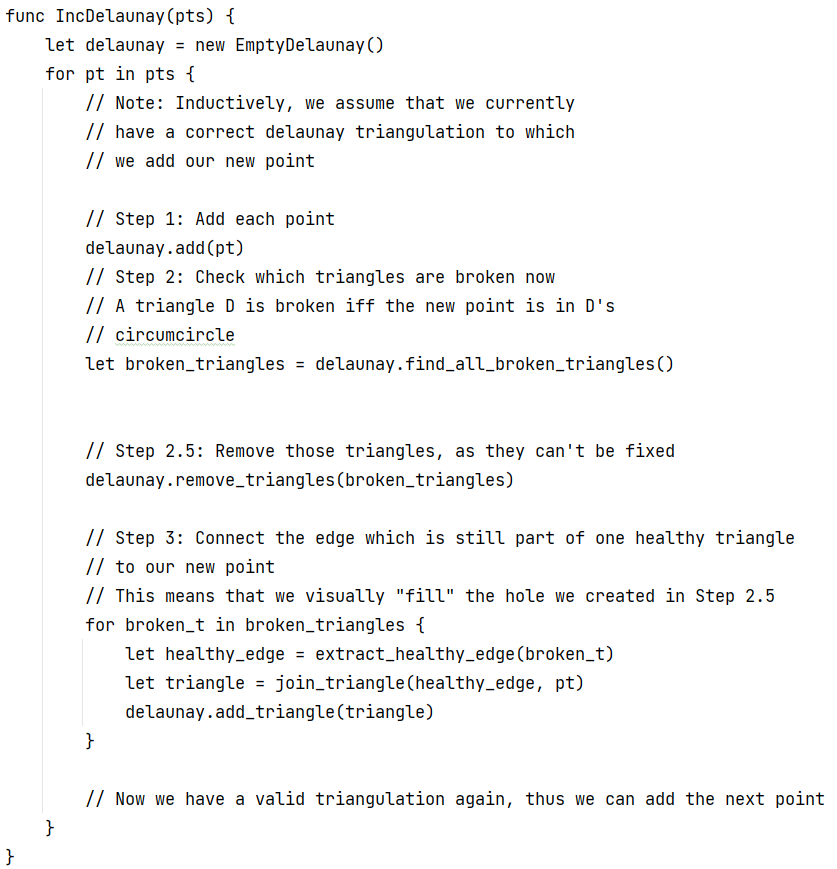
\includegraphics[width=\textwidth]{delaunayPseudocode.png}
    \caption{Pseudocode Green-Sibson/Bowyer/Watson}
    \label{fig:my_label}
\end{figure}
The average case time complexity is $O(n^{1 + 1/d})$ where $d$ is the number of dimensions \cite{Bowyer1981}.
% Runtime
\subsubsection{Divide and Conquer Algorithm}
A \textbf{Divide and Conquer} algorithm can be broken down into 3 steps:
\begin{enumerate}
    \item \textbf{Divide} the problem into smaller subproblems
    \item \textbf{Conquer} the subproblems by solving them recursively until they are small enough to be solvable straightforward.
    \item \textbf{Merge} the solutions of those smaller subproblems into the original problem
\end{enumerate}
This results in the following cost function
\[
T(n) := a\cdot T(n/b) + c(n)
\]
where
\begin{itemize}
    \item $a$ are the number of subproblems,
    \item $n/b$ is the size of the subproblem,
    \item $c(n)$ is the cost function matching the cost of the combine step.
\end{itemize}
This is equivalent to the following Pseudocode
\begin{figure}[H]
    \centering
    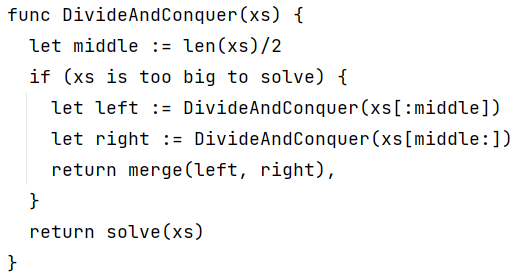
\includegraphics[width=0.7\textwidth]{pseudocode_dnc.PNG}
    \caption{Pseudocode D\&C}
    \label{fig:my_label}
\end{figure}
There are 2 ways to use the D\&C paradigm for constructing Delaunay Triangulations.
\newpage
The \textbf{naive way} would work as follows:
\begin{figure}[H]
    \centering
    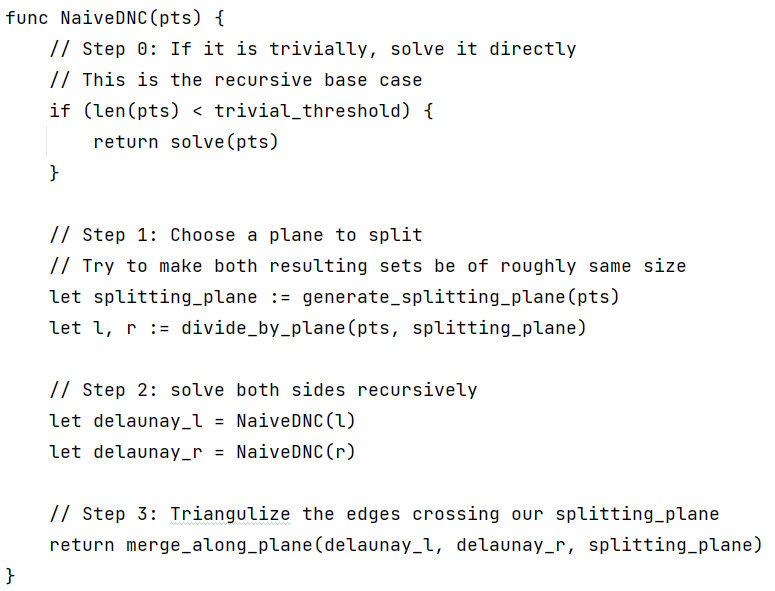
\includegraphics[width=\textwidth]{pseudocode_dnc_naive.PNG}
    \caption{Pseudocode D\&C for naively creating a Delaunay Triangulation}
    \label{fig:my_label}
\end{figure}
\begin{figure}[H]
     \centering
     \begin{subfigure}[b]{0.3\textwidth}
         \centering
         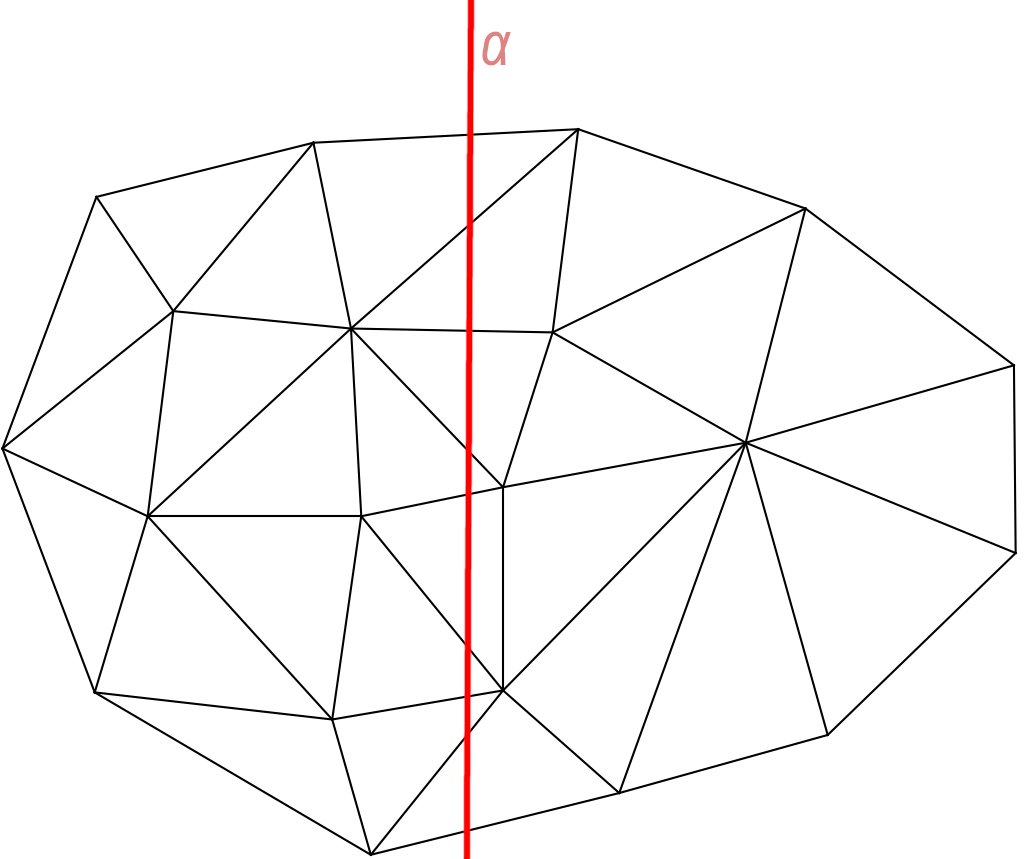
\includegraphics[width=\textwidth]{01NaiveCut.png}
         \caption{Divide into 2 subproblems}
         \label{fig:y equals x}
     \end{subfigure}
     \hfill
     \begin{subfigure}[b]{0.3\textwidth}
         \centering
         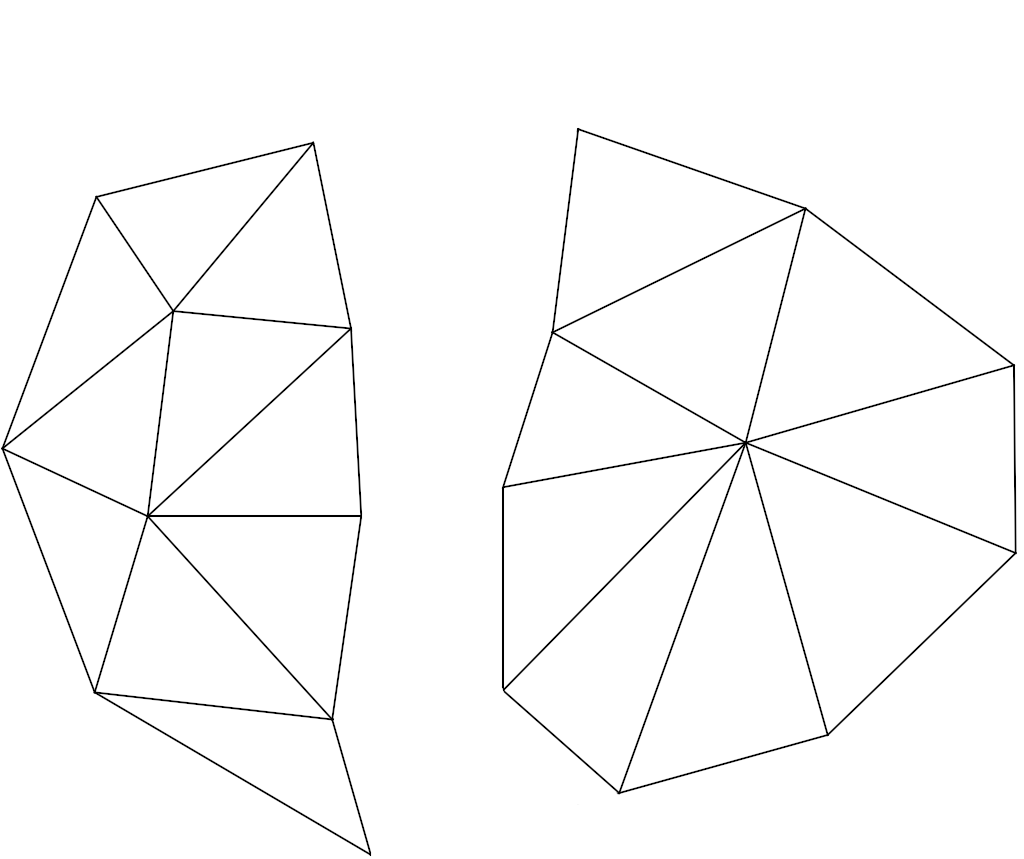
\includegraphics[width=\textwidth]{02NaiveSub.png}
         \caption{Solve the subproblems recursively}
         \label{fig:three sin x}
     \end{subfigure}
     \hfill
     \begin{subfigure}[b]{0.3\textwidth}
         \centering
         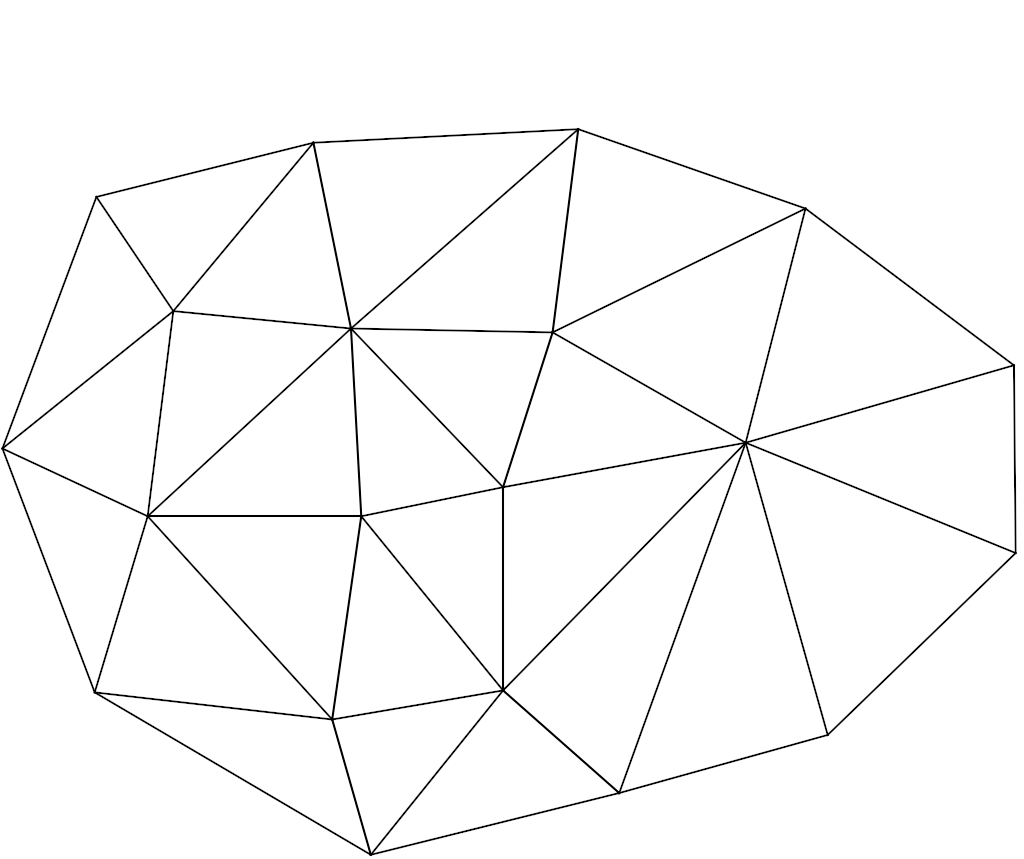
\includegraphics[width=\textwidth]{03SimpleConnectMiddle.png}
         \caption{Merge the subproblems}
         \label{fig:five over x}
     \end{subfigure}
        \caption{Naive D\&C Algorithm, Visually}
        \label{fig:three graphs}
\end{figure}
Note that, while merging both subproblems, this algorithm can still require additional changes to the already solved triangulations.\\
The better and more generalizable approach was first introduced by \cite{Cignoni1998}. The so-called \textbf{DeWall} algorithm can be simplified to the following idea:
\begin{figure}[H]
    \centering
    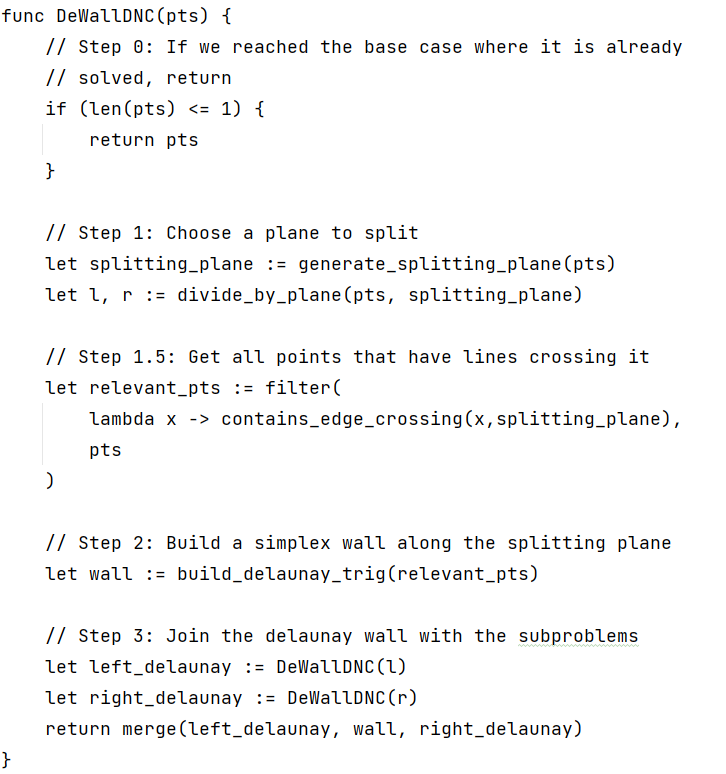
\includegraphics[width=\textwidth]{pseudocode_dnc_dewall.PNG}
    \caption{Pseudocode D\&C DeWall}
    \label{fig:my_label}
\end{figure}
\newpage
Visually:
\begin{figure}[H]
     \centering
     \begin{subfigure}[b]{0.3\textwidth}
         \centering
         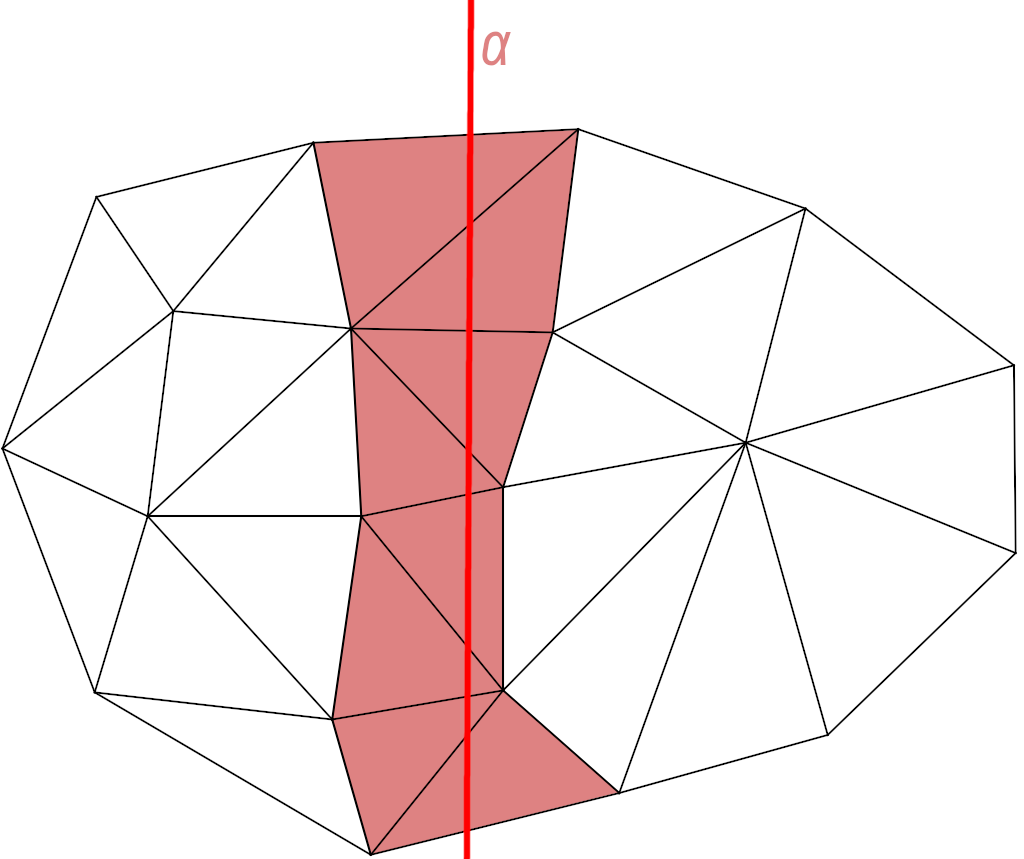
\includegraphics[width=\textwidth]{01DeWallMiddle.png}
         \caption{Cut into 2 problems}
         \label{fig:y equals x}
     \end{subfigure}
     \hfill
     \begin{subfigure}[b]{0.3\textwidth}
         \centering
         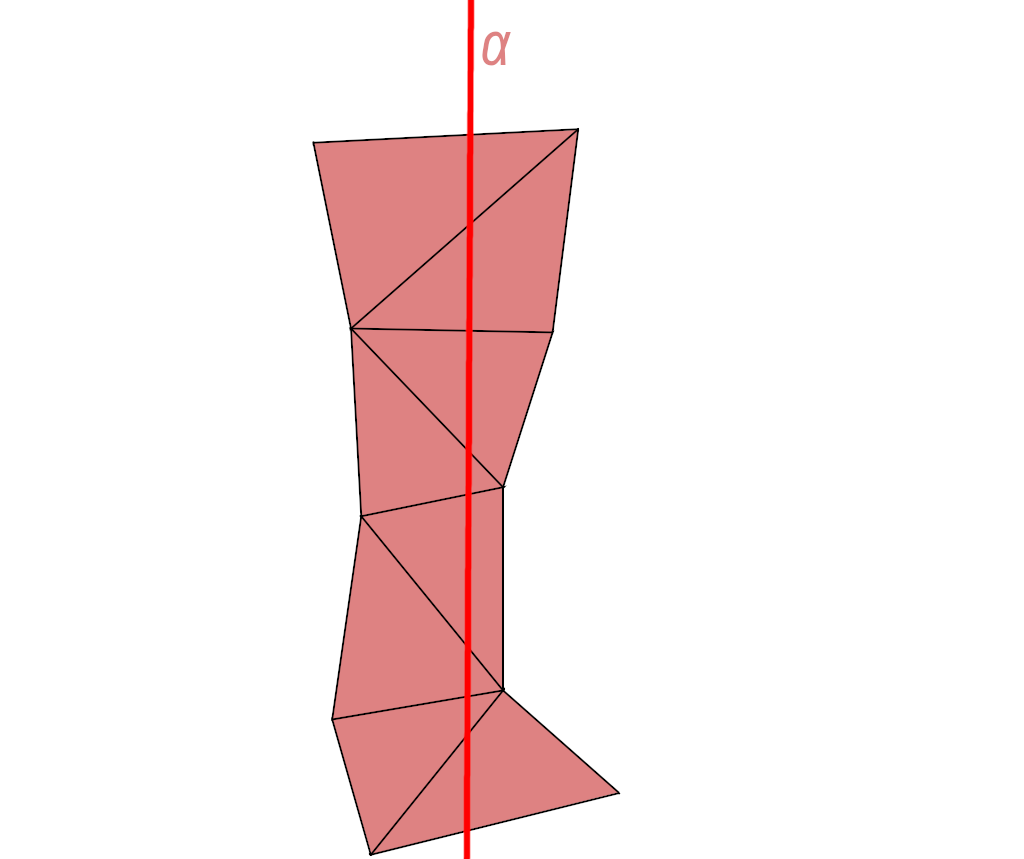
\includegraphics[width=\textwidth]{01DeWallSolveMiddle.png}
         \caption{Solve the Middle first}
         \label{fig:three sin x}
     \end{subfigure}
     \hfill
     \begin{subfigure}[b]{0.3\textwidth}
         \centering
         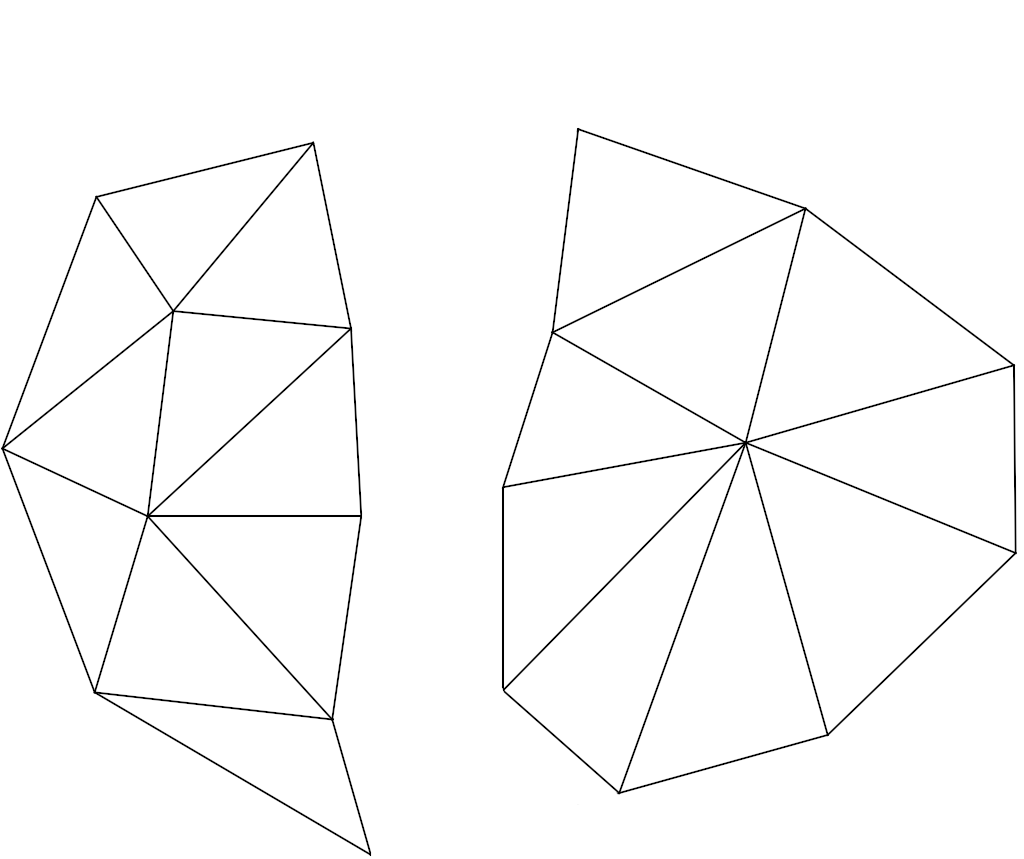
\includegraphics[width=\textwidth]{02NaiveSub.png}
         \caption{Solve the both sides recursively like (ii)}
         \label{fig:five over x}
     \end{subfigure}
        \caption{DeWall Algorithm, Visually}
        \label{fig:three graphs}
\end{figure}
The worst case time complexity of DeWall is known to be $O(n^{\lceil d/2 \rceil +1})$, with $d$ being the number of dimensions
\subsubsection{S-hull Algorithm}
The \textbf{S-hull} \cite{Sinclair2010} algorithm belongs to the family of the so-called line sweep algorithms, which describes solving a problem geometrically in an space by traversing it and working with distances. Note that this requires an euclidean norm.\\
\cite{Sinclair2010} contains a great pseudocode summary:
\begin{quote}
    S-hull operates as follows: For a set of unique points $x_i \in \mathbb{R}^2$:
    \begin{enumerate}
        \item select a seed point $x_i$ from $x_i$.
        \item sort according to $|x_i - x_0|^2$.
        \item find the point $x_j$ closest to $x_0$.
        \item find the point $x_k$ that creates the smallest circum-circle with $x_0$ and $x_j$ and record the center of the circumcircle $C$.
        \item order points $[x_0, x_j, x_k]$ to give a right handed system: this is the initial seed convex hull
        \item resort the remaining points according to $|x_i-C|^2$ to give points $s_i$.
        \item sequentially add the points $s_i$ to the porpagating 2D convex hull that is seeded with the triangle formed from $[x_0, x_j, x_k]$. As a new point is added the facets of the 2D-hull that are visible to it form new triangles.
        \item a non-overlapping triangulation of the set of points is created. (This is an extremly fast method for creating an non-overlapping triangulation of a 2D point set).
        \item adjacent pairs of triangles of this triangulation must be 'flipped' to create a Delaunay triangulation from the initial non-overlapping triangulation.
    \end{enumerate}
\end{quote}
This algorithm just works on 2D and it's worst case time complexity is $O(n\log n)$. 
\subsubsection{q-hull Algorithm}
\begin{definition}[Convex Set]
A Set $S$ is \textbf{convex} if, for all $x,y \in S$, the line segment $L_{x,y} := \{ tx+(1-t)y : t \in [0,1] \}$ is in $S$.
\end{definition}
\begin{definition}[Convex Hull]
A \textbf{Convex Hull} of a set of $N$ points is defined as the smallest convex set which contains all of the points.
\end{definition}
In $\mathbb{R}^2$, this is a convex polygon of at most $N$ sides.\\
\begin{theorem}[Delaunay Triangulation/Convex Hulls]
A Delaunay triangulation in $\mathbb{R}^d$ can be created by computing the convex hull in $R^{d+1}$, followed by then extracting the set of ridges of the lower convex hull.
\end{theorem}
\begin{proof}
Constructive proof, see \cite{Brown1979}.
\end{proof}
This is the most common way for computing Delaunay triangulation, as most numerical libraries like Scipy \cite{Scipy2022} use the qhull library \cite{QHull} based on the Quickhull Algorithm \cite{Barber1996}.
\subsection{Our Algorithm and Implementation}
We chose to implement an incremental algorithm which is a simplified version of \cite{Green1978}, which in itself is a $2$ dimensional version of \cite{Bowyer1981} and \cite{Watson1981}, in which finding the triangle containing a new point takes $O(n)$, instead of the $O(\sqrt{n})$ neighbour walk alleged by \cite{Bowyer1981}.
\subsubsection{Basic Idea}
As mentioned before, all incremental algorithms work inductively by assuming a valid Delaunay triangulation of $n-1$ points, adding the $n$-th point, then repairing the triangulation afterwards.
\newpage
\cite{Rebay1993} summarizes the algorithm as follows:
\begin{quote}
    The method is based on the so-called \textit{circumcircle property} which guarantees that no point of a Delaunay triangulation can lie within the circle circumscribed to any triangle. The Bowyer-Watson algorithm is essentially a "reconnection" method, since it computes how an existing Delaunay triangulation is to be modified because of a new point.
\end{quote}
\subsubsection{A visual example}
Assume we have generated the following valid Delaunay triangulation of $n-1$ points:
\begin{figure}[H]
    \centering
    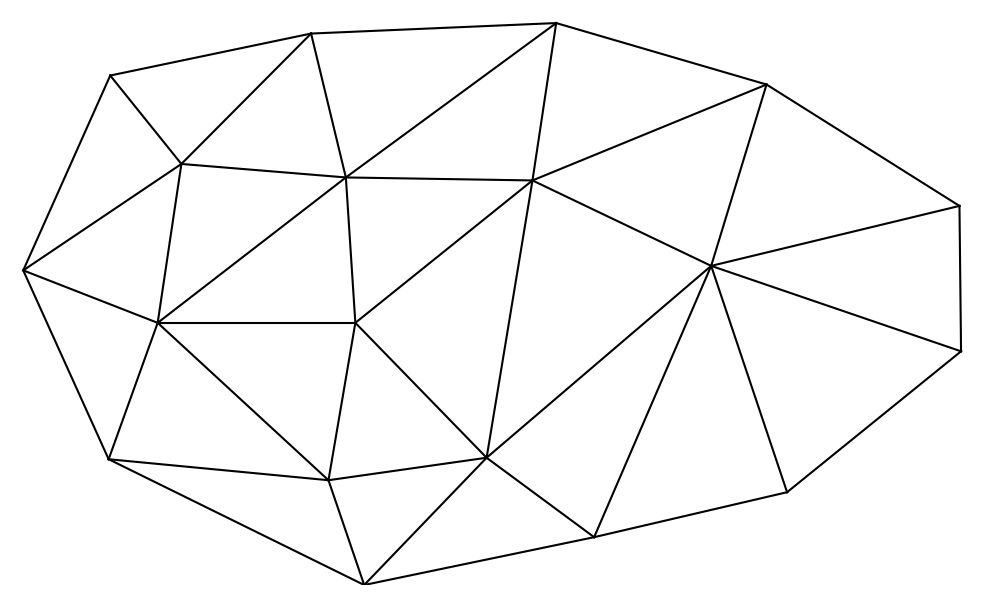
\includegraphics[width=0.6\textwidth]{DelaunayVisualExample01.png}
\end{figure}
Now we want to add a new point into this triangulation.
\begin{figure}[H]
    \centering
    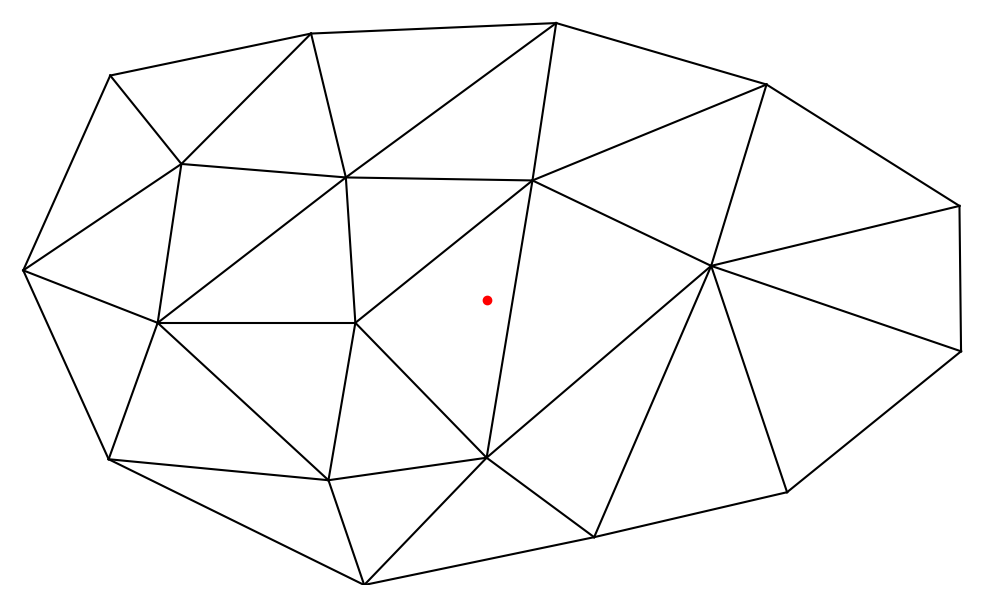
\includegraphics[width=0.6\textwidth]{DelaunayVisualExample02.png}
\end{figure}
The circumcircle property shows us that any valid Delaunay triangulation has no other points in the circumcircles spanned by all triangles. This also means that any triangle that contains our new point can't be valid!\\
Note that we just have to focus on our newly inserted point since we know that we started with an already valid Delaunay triangulation.
\newpage
Let's look at the circumcircles:
\begin{figure}[H]
    \centering
    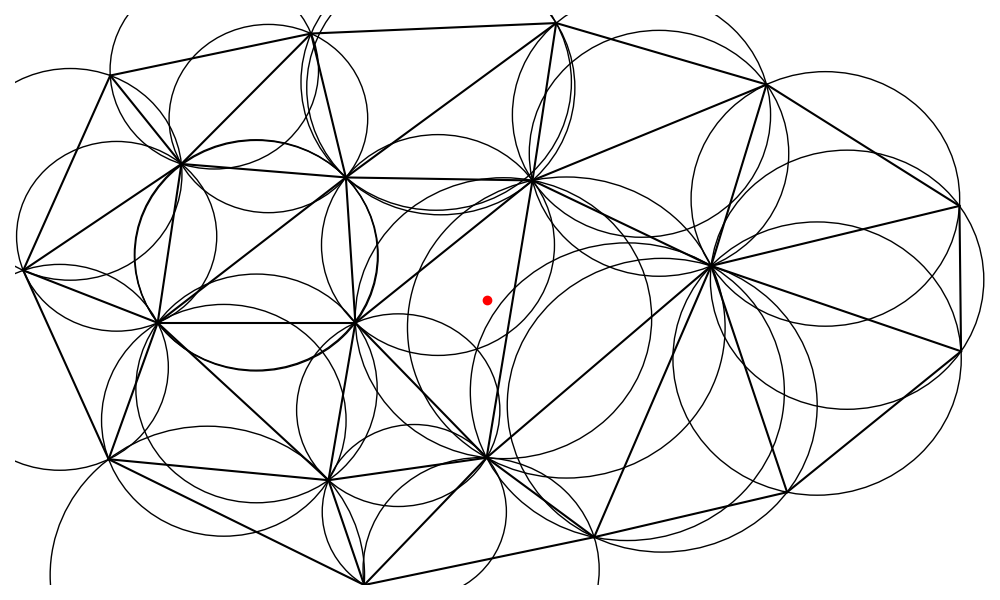
\includegraphics[width=0.6\textwidth]{DelaunayVisualExample03.png}
\end{figure}
Now just show the invalid ones:
\begin{figure}[H]
    \centering
    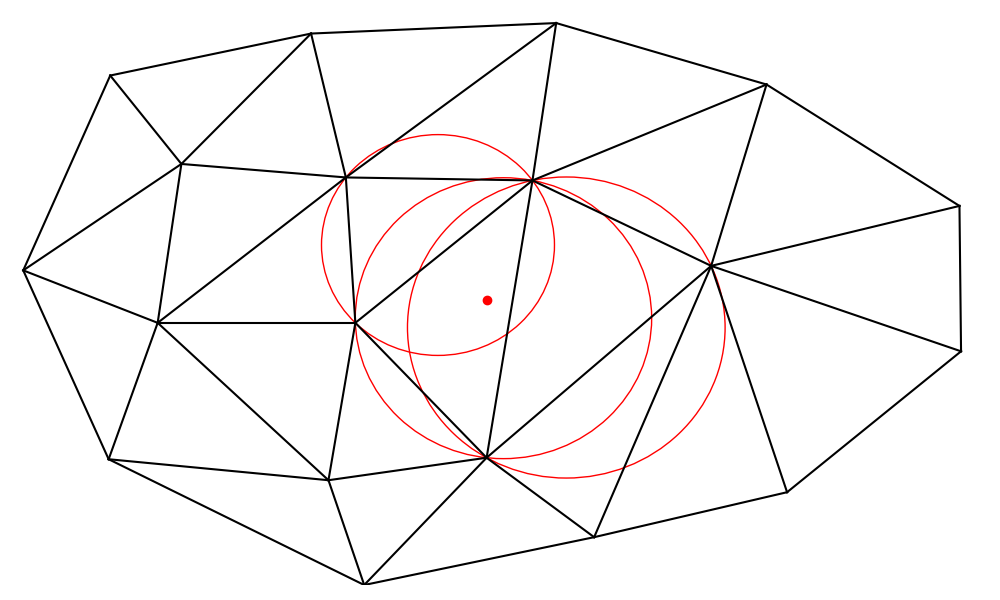
\includegraphics[width=0.6\textwidth]{DelaunayVisualExample04.png}
\end{figure}
We now know that those triangles are broken. Thus we remove them.
\begin{figure}[H]
    \centering
    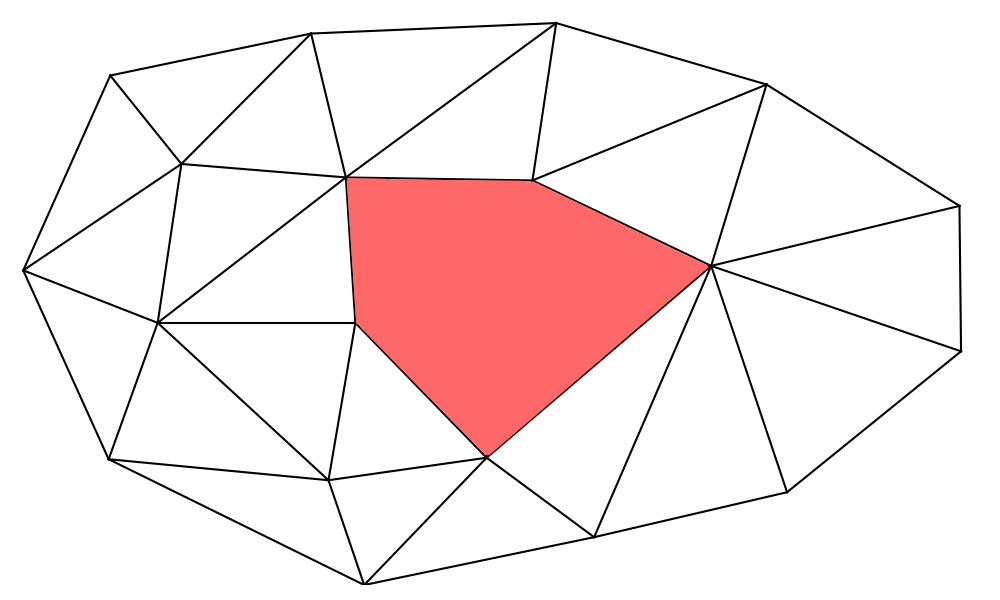
\includegraphics[width=0.6\textwidth]{DelaunayVisualExample05.png}
\end{figure}
Now we only have one valid way to fill the hole: Connecting all leftover edges to our new point. This makes sense intuitively, since this way results in the most equilateral triangles, thus furfilling Delaunay's optimality criteria. Formally, we know that a triangulation is Delaunay if and only if it is locally Delaunay, which means that any non-optimal solution wouldn't be possible (\cite{FORTUNE1995}, Lemma 2.2).\\
So let us reconnect them:
\begin{figure}[H]
    \centering
    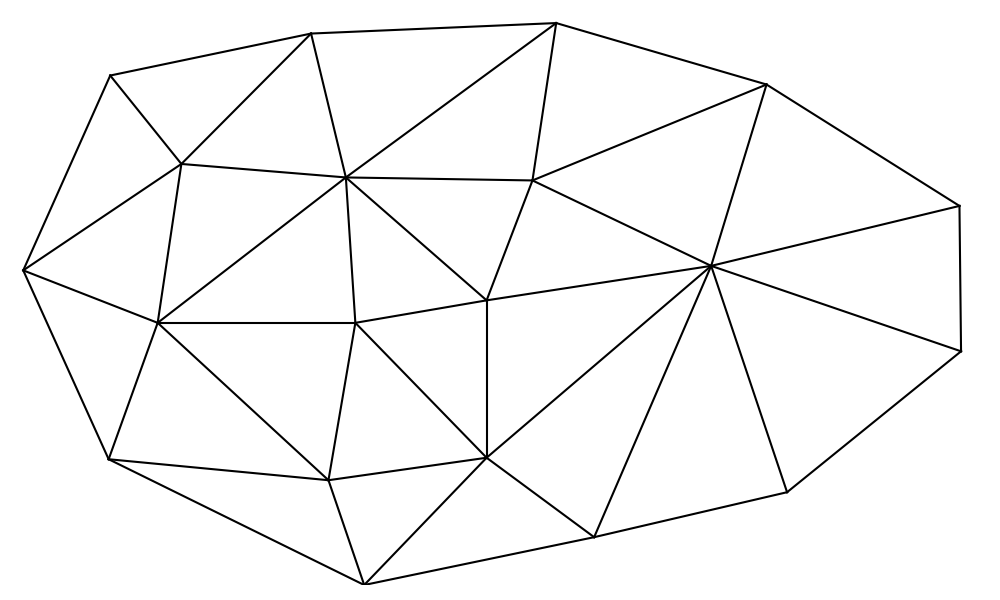
\includegraphics[width=0.6\textwidth]{DelaunayVisualExample06.png}
\end{figure}
Now we have a valid triangulation of $n$ points. To verify, here are all circumcircles:
\begin{figure}[H]
    \centering
    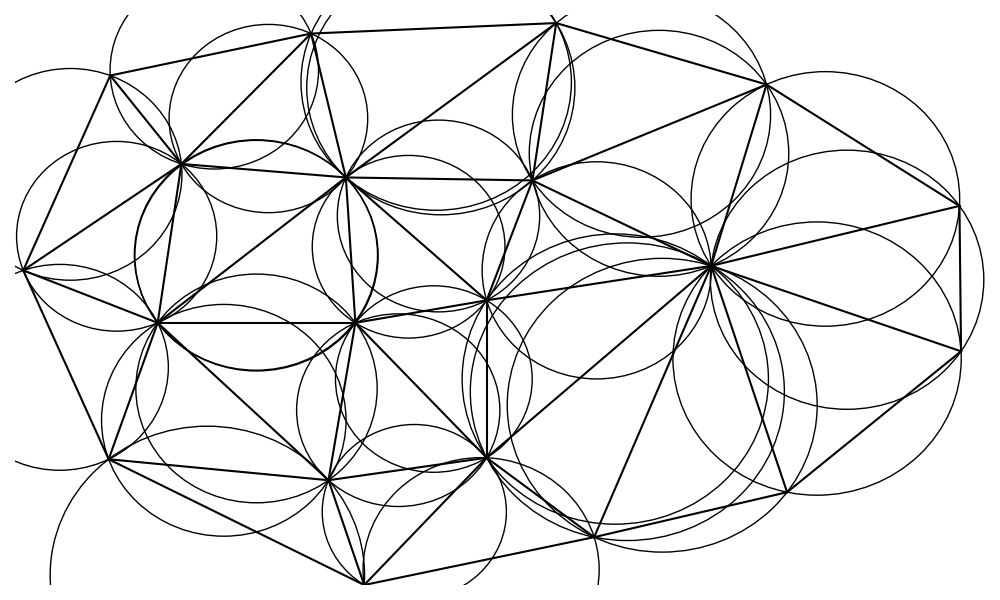
\includegraphics[width=0.6\textwidth]{DelaunayVisualExample07.png}
\end{figure}
And for clarity, just the new circumcircles:
\begin{figure}[H]
    \centering
    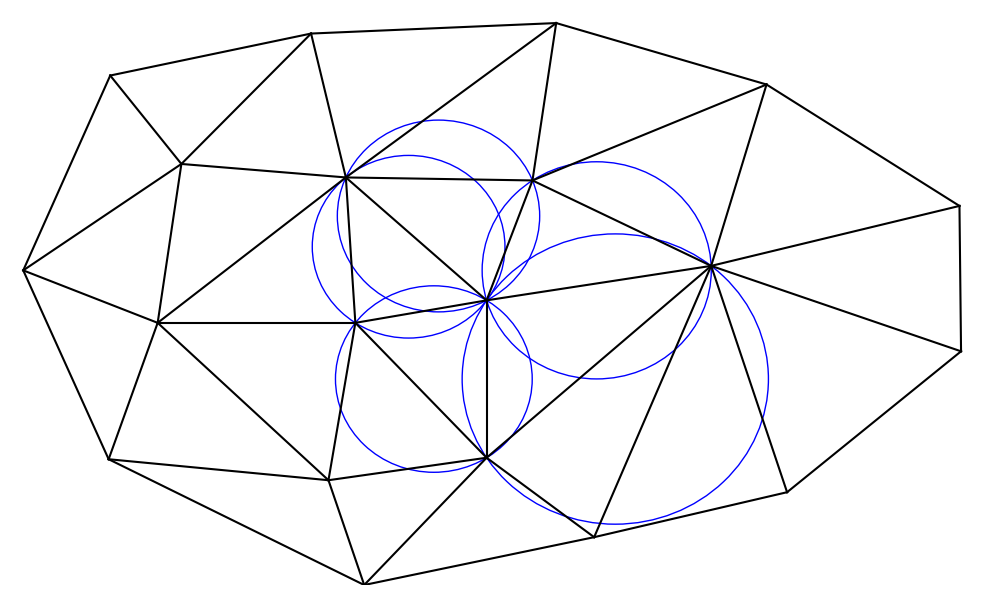
\includegraphics[width=0.6\textwidth]{DelaunayVisualExample08.png}
\end{figure}
Now all are valid again, resulting in a new Delaunay triangulation
of $n$ points.
\subsubsection{Initial State}
The incremental method works inductively and as we have just seen our induction step is correct. Now we have to handle the base case. This is more difficult because any set with less than 3 points is not triangularizable.\\
In order to make it easier, we use Green-Sibson's window \cite{Green1978} and extend it with a supertriangle \cite{PyDelaunay}.
\begin{definition}[Window]
A \textbf{window} is a axially parallel rectangle which contains all points of the Delaunay triangulation.
\end{definition}
Now we also have to extend our Voronoi tile definition:
\begin{definition}[Window-aware Voronoi tiles]
Let $\mathcal{P}_N := \{P_1,\dots, P_N\}$ be finitely many points in the plane such that $P_i \neq P_j, i \neq j$.  Further let $E$ be a window such that all points fit. The \textbf{window-aware Voronoi tile} of $P_i$ is the set $T_i^*$ defined by
\[
T_n^* := \{ x \in E : d(x, P_i) < d(x, P_j) \forall i \neq j, P_j \in E  \}
\]
In our algorithm, all Voronoi tiles are window-aware.
\end{definition}
The window used in our algorithm is square. This window allows us to have a boundary, in which all points are contained. In order to make the window a valid triangulation we extend it to a super-triangle:
\begin{definition}[Supertriangle]
A \textbf{supertriangle} is a window with an additional diagonal edge, dividing it into 2 triangles.
\end{definition}
\begin{figure}[H]
    \centering
    
\includegraphics[width=0.5\textwidth]{supertriangle.png}
    \caption{Supertriangle, all points outside of it are invalid}
    \label{fig:my_label}
\end{figure}
This supertriangle is only used internally; all edges and vertices are not part of the Delaunay triangulation.
\subsubsection{Mesh Data Structure}
The most important part of this algorithm is fast graph traversal, thus we heavily rely on a efficient mesh data structure. Our data structures are defined as follows:
\begin{figure}[H]
    \centering
    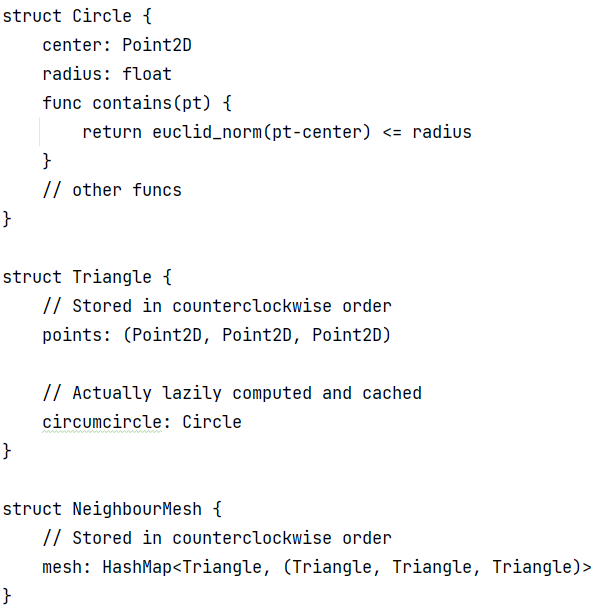
\includegraphics[width=\textwidth]{ds.png}
\end{figure}
The Mesh gets updated while adding new points.\\
This Data structure has multiple great properties:
\begin{itemize}
    \item Since we only have 2 dimensions and have the circle as a member variable, detecting whether a point lies in a triangles circumcircle is $\Theta(1)$.
    \item Although Python dictionaries (i.e. Hashmaps) use open hashing, our hash function is chosen in a way that the hash seed of two triangles is only equal if and only if they share all 3 points. Thus our triangle lookup results in $\Theta(1)$.
    \item Since any triangle only has 3 neighbours, we can traverse $n$ triangles in $\Theta(n)$, which is obviously optimal.
\end{itemize}
\subsubsection{Triangle Replacement Optimization}
In order to optimize the triangle replacement we use 2 useful properties from \cite{Rebay1993}:
\begin{quote}
    The algorithm removes from the existing grid all the triangles which violate the circumcircle property because of the insertion of the new point.\\
    It can be shown that
    \begin{enumerate}
        \item all these triangles are always contiguous, thus forming a connected cavity surrounding the newly inserted point, and that
        \item by joining the vertices of the cavity with the internal new point, a Delaunay triangulation is always obtained.
    \end{enumerate}
\end{quote}
Our optimization thus consists of three parts:
\begin{itemize}
    \item The aforementioned $O(1)$ traversal neighbour mesh data structure
    \item Remembering which edges need to be reconnected while deleting the broken triangles
    \item Only traversing along the hole edges, starting at a random edge. This works because we know that the hole is contiguous.
\end{itemize}
\newpage
\subsubsection{Triangle Replacement Implementation}
This is the code for adding a new point to the Delaunay triangulation:
\begin{figure}[H]
    \centering
    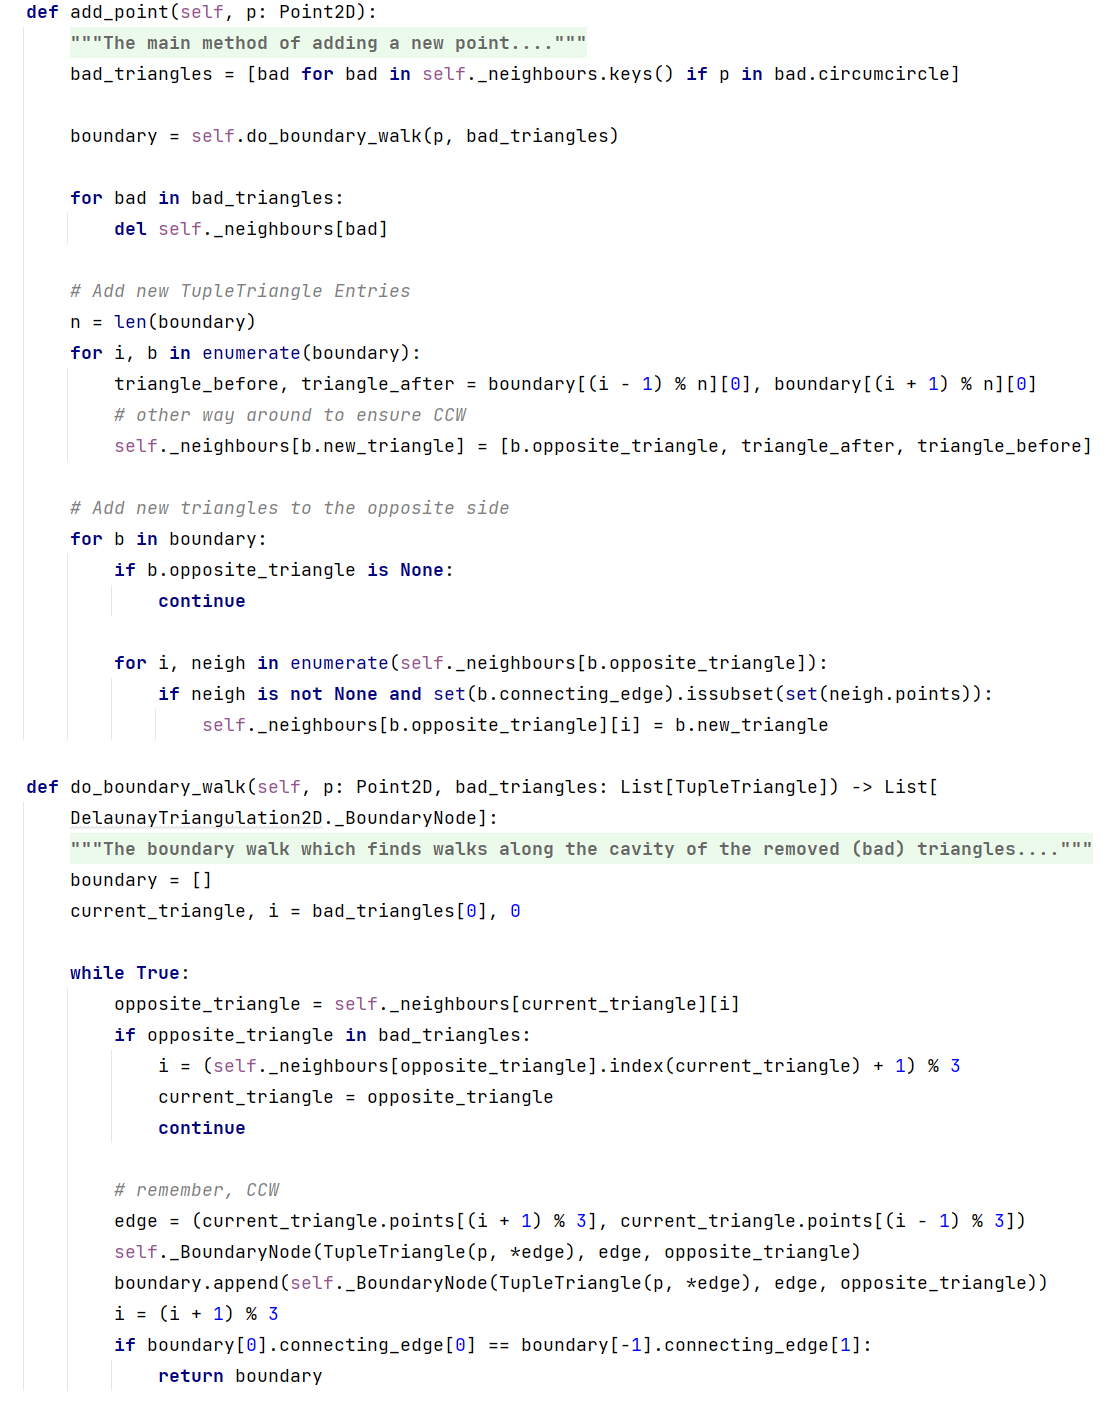
\includegraphics[width=\textwidth]{add_point_full.png}
\end{figure}
It works as follows:
\begin{itemize}
    \item At first, we detect all broken triangles by checking their circumcircles
    \item Now we do the \textbf{boundary walk} that works as follows:\\
    We start at any triangle. Note that we cannot yet know whether it is entirely surrounded by broken triangles or not. We choose any edge of it.\\
    Then we rotate along the edges counter clock wise (CCW) and go to the triangle that is connected to our triangle through this edge. One can see that through this motion we go in a more or less specific direction.\\
    Eventually (in reality it's pretty fast, \cite{Green1978} shows that through the Euler-Poincare formula) we reach an edge that is connected to a valid triangle (i.e. a triangle which circumcircle contains only it's 3 points). This is relevant because we have to reconnect the edge connecting the broken and valid triangle to our new point.\\
    We call this edge-path of valid-to-invalid triangles our \textbf{boundary}.\\
    Now, by moving counter clock wise, we stay along the boundary. We record not only every boundary edge, but also to which boundary edges it is connected to. This allows for linear time insertion of the new triangles since we do not have to search the neighbour (which, combinatorically, would result in $O(n^2)$ where $n$ is the number of boundary edges).
    \begin{figure}[H]
    \centering
    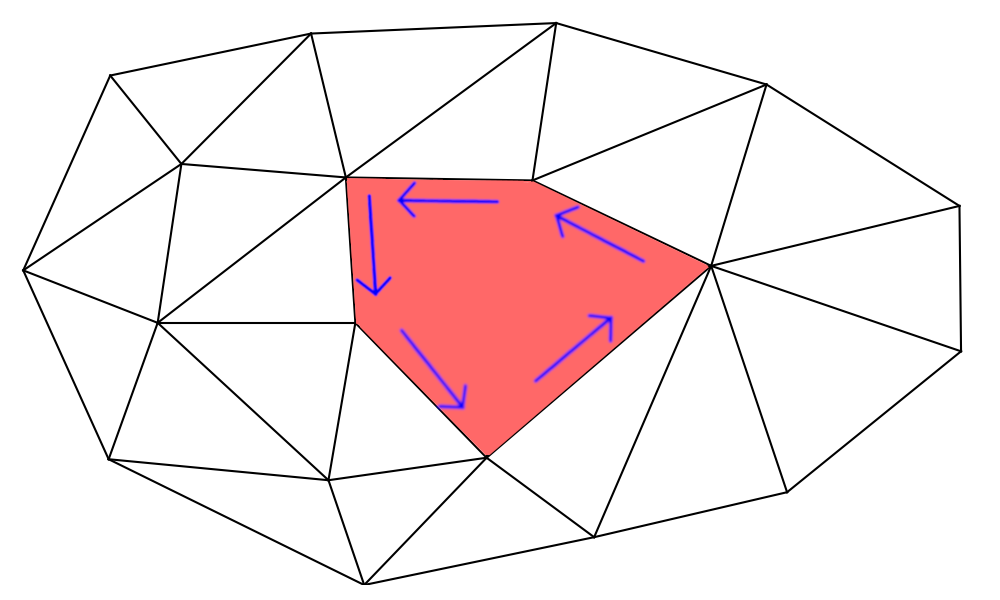
\includegraphics[width=0.5\textwidth]{ccwBoundaryWalk.png}
    \caption{CCW walk. We always check that we are connected to one valid and one broken triangle}
    \label{fig:my_label}
    \end{figure}
    Note: the neighbours do not have to be saved explicitly. Since it is a list, and we add it one by one while walking along the neighbourship, it is implicitly ordered.\\
    We stop once we meet our first boundary triangle again (we ran a circle).\\
    \textit{This is the main algorithm optimization}.
    \item After collecting the boundary, we can delete all broken triangles.
    \item Lastly, we walk along the boundary and create new triangles, consisting the boundary edge connected to our new point. Note that we can add the triangle neighbours in $O(1)$ because our boundary is ordered (see the traversal).
\end{itemize}
\subsection{Runtime Analysis}
The initial data structure creation is $\Theta(1)$. For each point, we have the following costs for adding the $n$-th point:
\begin{enumerate}
    \item To detect all broken triangles, we look at all triangles. As explained in the data structure section, this lookup is $\Theta(1)$, resulting in $\Theta(n)$
    \item The boundary walk takes $\Theta(1)$ per triangle. Thus we can choose an upper bound of $O(n)$, although this bound is not very tight.
    \item Deleting a bad triangle takes $\Theta(1)$. Thus $\Theta(1) \cdot |\text{\texttt{bad\_triangles}}| \in O(n)$.
    \item Connecting one boundary edge with the new point, creating a new triangle and updating our neighbour mesh all takes $\Theta(1)$. Again, its upper bound is $O(n)$
\end{enumerate}
Resulting in a runtime of $\Theta(n) + 3 \cdot O(n) = O(n)$ per point.\\
If we have $m$ points, this results in $O(m^2)$.
\subsubsection{Possible Improvements and Beyond}
As shown by Bowyer-Watson \cite{Bowyer1981} \cite{Watson1981}, this algorithm could theoretically be generalized to $n$ dimensions.\\
Both Green-Sibson \cite{Green1978}, Bowyer \cite{Bowyer1981} and \cite{Rebay1993} alledge that the nearest-neighbour search (i.e. finding the triangle our new point is contained in) can be implemented in $O(n^{1/d})$ with $d$ being the dimension. Sadly, this was never proven rigorously \cite{FORTUNE1995}. Also, no algorithm is mentioned in the literature. For now, the question on whether this is actually possible remains open \cite{CSSE}.



\newpage
\printbibliography
\end{document}
